\documentclass[12pt, a4paper, ngerman]{article}

%\usepackage{fancyhdr,graphicx, fleqn}
\usepackage{graphicx}
\usepackage[ngerman]{babel}
\usepackage[utf8]{inputenc}
\usepackage[T1]{fontenc}
\usepackage{amsmath}
\usepackage{lmodern} 
\usepackage{acronym} 
\usepackage{tikz}



\setlength{\parindent}{0pt} %Absätze nicht einrücken




\begin{document}
\tableofcontents
\section{Einleitung}
%

Im Abschnitt Motivation  wird definiert, warum es Sinn macht, Ger"ate z.b Kompressor 
im Industrie 4.0 zu vernetzen.Es wird zuerst die technische L"osungen gezeigt. 
Im Abschnitt Zielsetzung wird erkl"art, was man mit dieser Arbeit 
erreicht wird und welche Bestandteil daf"ur benutzt wird.
\subsection{Zusammenfassung}

Industrie 4.0 ist das Schlagwort,welches die 4.Industrielle Revolution beschreibt.
Ger"ate und Maschinen werden heute Intelligent durch die Vernetzung miteinander und
 mit den Menschen "uber das Internet kommunizieren.
Maschinen und Ger"ate werden in der Zukunft digitalisiert 
\footnote{Digitalisierung bedeutet in dieser Arbeit die Vernetzung der einzelnen Komponenten untereinander.} 
und mit Sensoren aufgebaut sein.
Sie kommunizieren immer mit verschiedenen Systemen.
 Zum Beispiel mit
Entwicklung, Produktion  sowie Lieferanten und Kunden.
Damit das alles funktioniert, m"ussen Sensoren in Maschinen
digital erfasst werden. Es gibt einen neuen Begriff,
der das Internet of Things (IoT) hei"st, um die Sensoren
und andere Maschinen mit digitalen Informationen zu verbinden.
Die Bewertung und Simulationen werden "uber das Internet funktionieren.
Dank der Vernetzung in der Industrie 4.0 k"onnten Menschen viele
genaue Informationen von verschiedenen Quellen erhalten und falls
es St"orungen gibt k"onnten diese schnell bearbeitet werden und gleichzeitig 
die richtigen Entscheidungen getroffen werden. 
Diese Entwicklung verbessert viele Prozesse in unterschiedlichen
Bereichen und vereinfacht die Kommunikation mit anderen Abteilungen.[1]
\subsection{Zielsetzung}

Das Ziel dieser Arbeit ist die Konzeption und Entwicklung einer
mechatronischen Betriebsumgebung f"ur einen Kompressoren-Versuchsstand
in Anlehnung an Industrie 4.0.
Daf"ur soll ein mechatroniches Konzept und Auswertunggsoftware 
entwickelt werden.Das Auslesen der Sensoren erfolgt "uber einen Arduino,
mit der Plattform eigenen Programmiersprache.Die Auswertung der Daten 
soll dann mit Hilfe von PHPausgewertetund mit MYSQL gespeichert werden.Die
Auswertung soll dem Anwender anschlie"send grapisch zur Verf"ugung stehen.
 

Das Layout folgt in den Kapiteln Projektplanung, Software Engineering
und UI-Prototypen. Weil Software Engineering grundlegend f"ur die
Software-Entwicklung ist und die Nutzbarkeit Hand in Hand mit der
Software-Entwicklung funktioniert, deswegen ist es wichtig,
sich eingehend mit dem Entwicklungs-Modell/Prozess zu befassen.



\section{Stand der Technik}
\subsection{Einsatz und Aufbau von Kompressoren}
Die Aufgabe von Kompressoren ist es Gase zu komprimieren.
In diesem Fall nimmt die Dichte der Gase zu, gleichzeitig wird das
Volumen verkleinert.
Dar"uber hinaus steigen die Temperatur und der Druck durch die resultierte
Kraft, die gebraucht wird, um die Gase entgegen ihres nat"urlichen
Verhaltens zu verdichten. [2] 
Es gibt zwei Arten von Kompressoren, einen Kolbenkompressor
und einen Schrauben-Kompressor. 
In der Arbeit wird ein Kolbenkompressor benutzt,
auf diese Bauweise n"aher eingegangen.Den Aufbau eines typischen
Kolbenkomprerssor sehen Sie in Abbildung~\ref{fig:komp1}.

\begin{figure}[!htb]
\begin{center}
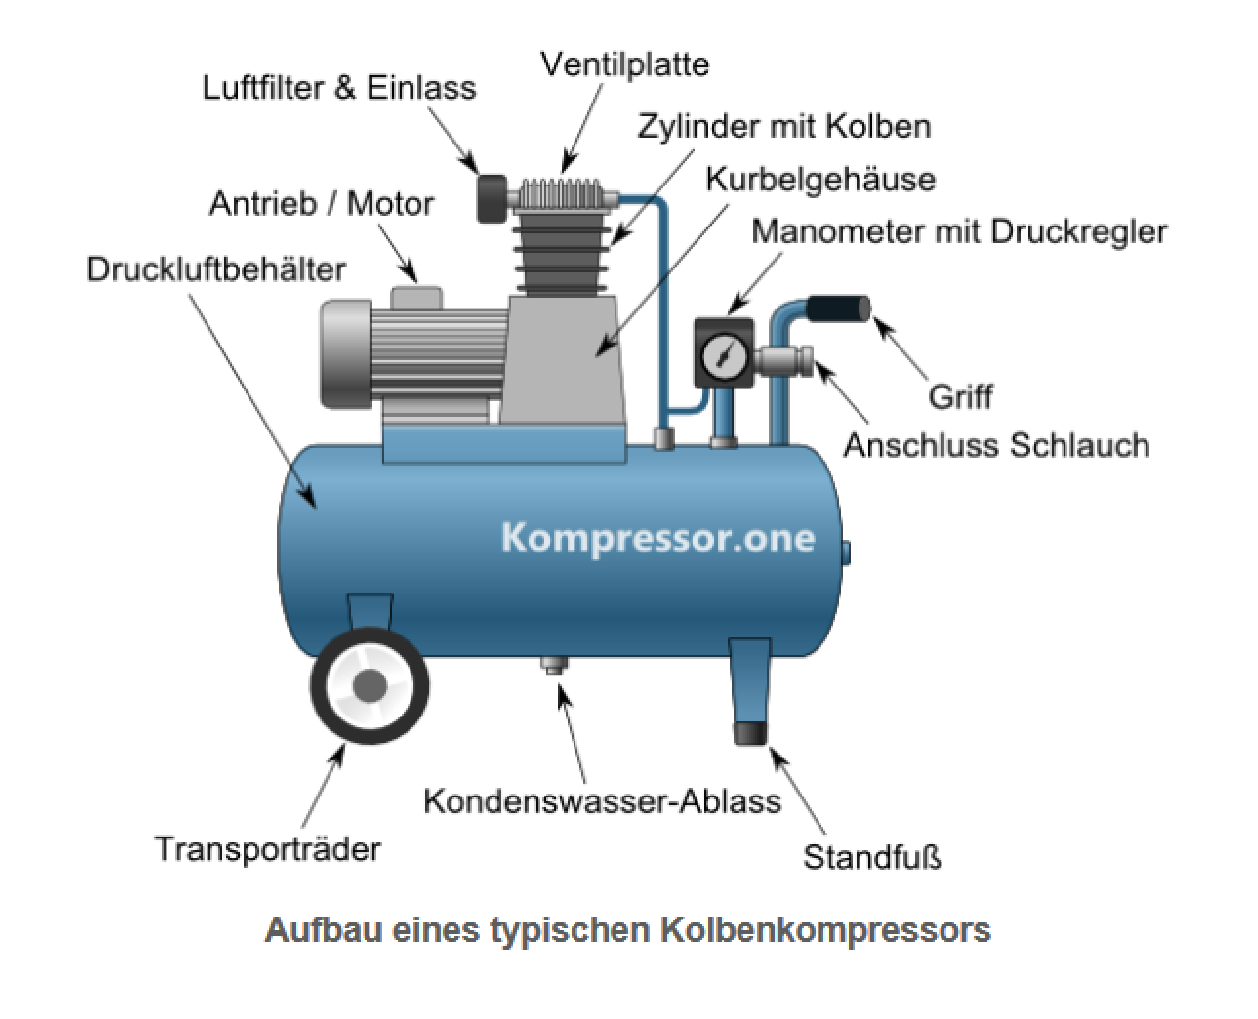
\includegraphics[height=7cm]{bilder/Kompressor.eps}
\end{center}
\caption{Aufbau eines typischen Kompressors}\label{fig:komp1}
\end{figure}

Sobald der Kolbenverdichter in Betrieb ist,
wird sich der Kolben,
der mit einer Dichtung zur Zylinderwand hin abgedichtet ist, 
hin und her bewegen. 
Wenn sich der Kolben zurückzieht, 
wird Luft durch das Einlassventil wie gezeigt in Abbildung~\ref{fig:komp2} angesogen 
und wenn sich der Kolben wieder vorschiebt, 
schlie"st sich dieses Ventil  
 und die Luft wird zusammengedrückt 
und wiederum wie gezeigt in Abbildung~\ref{fig:komp3} durch das Auslassventil abgegeben.


\begin{figure}[!htb]
\begin{center}
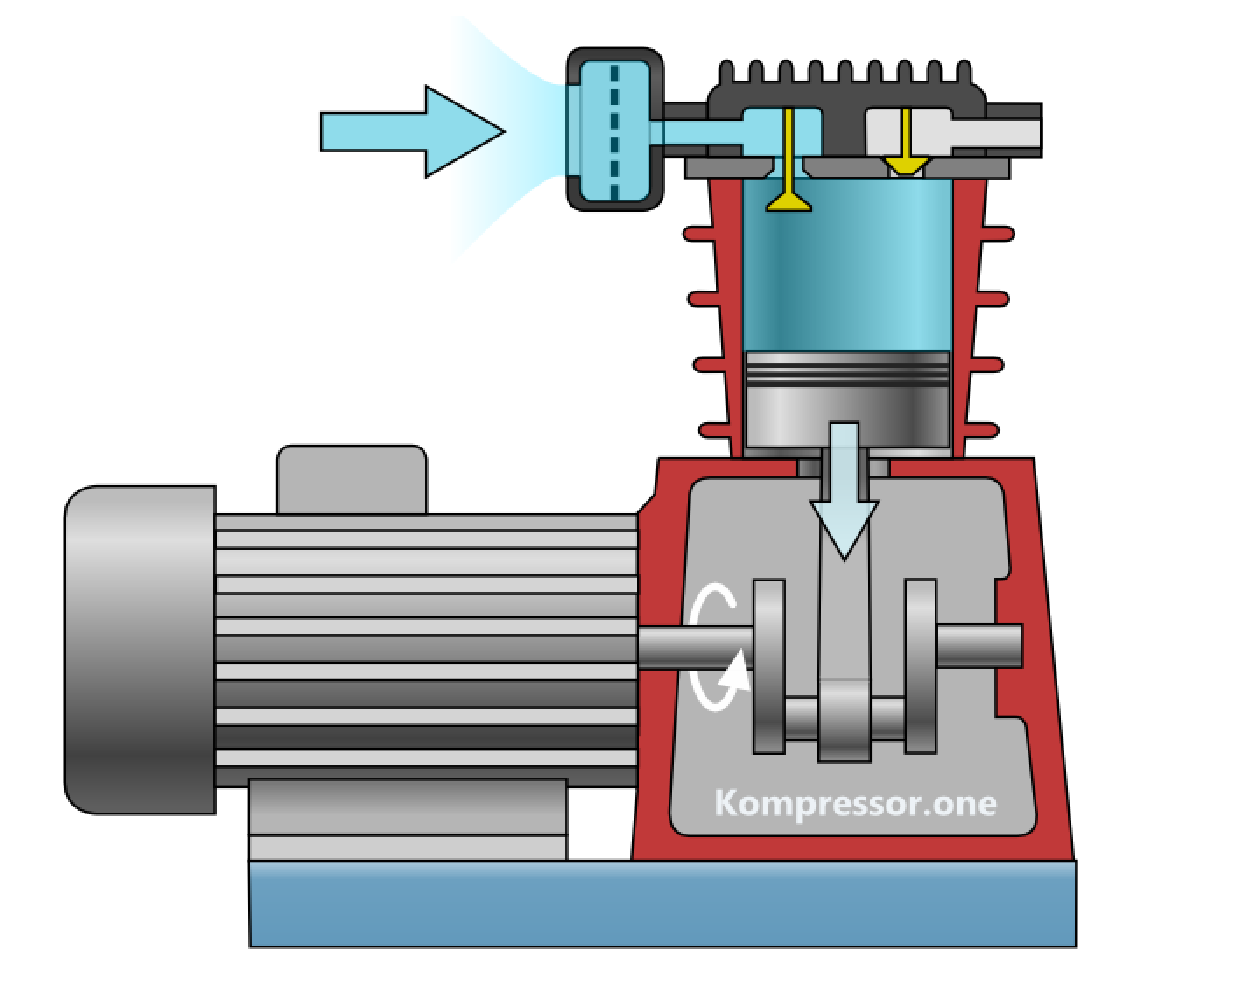
\includegraphics[height=7cm]{bilder/Kom2.eps}
\end{center}
\caption{Ansaugen}\label{fig:komp2}
\end{figure}

\begin{figure}[!htb]
\begin{center}
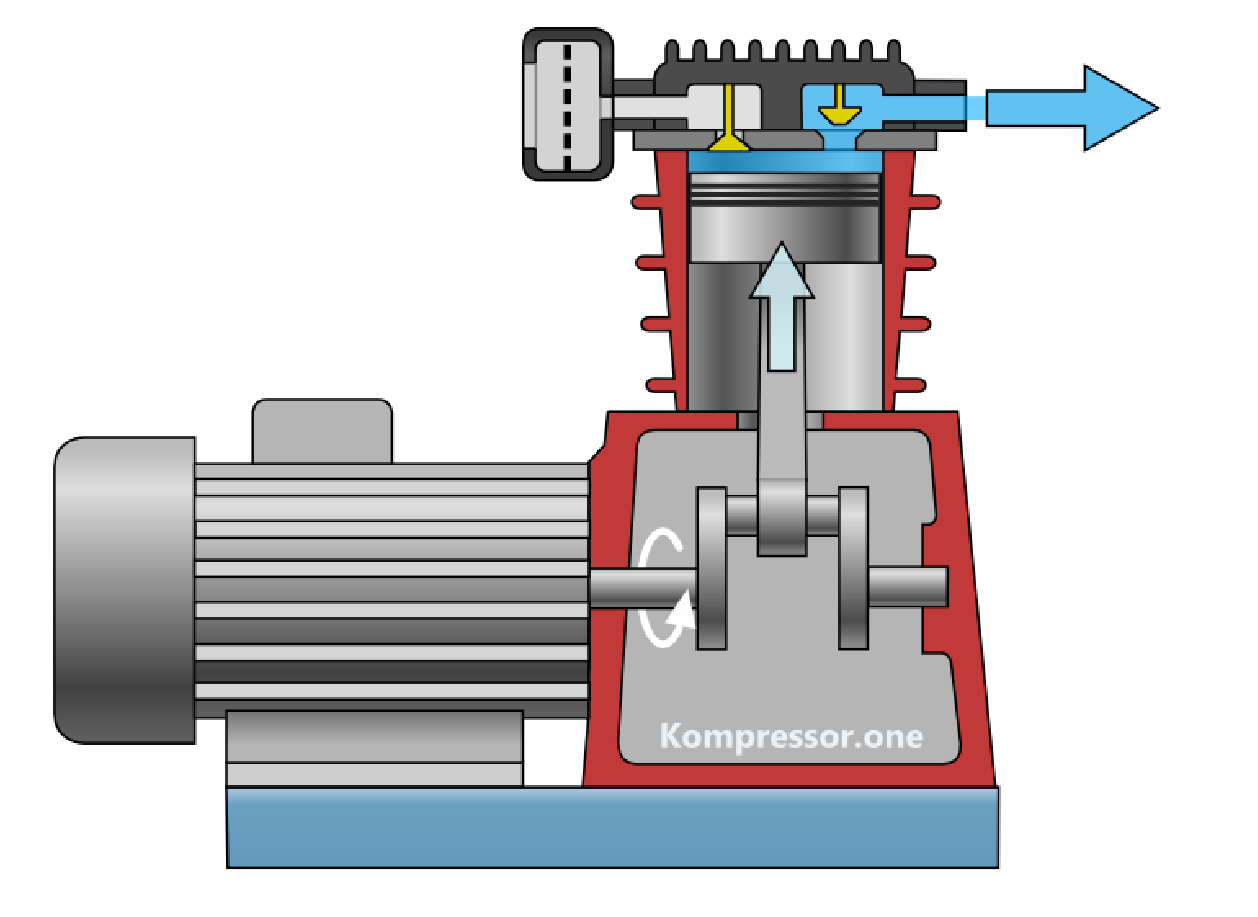
\includegraphics[height=7cm]{bilder/kom3.eps}
\end{center}
\caption{Verdichten}\label{fig:komp3}
\end{figure}

Der Aufbau und das Prinzip des Kolbenkompressors "ahnelt 
sehr einer handels"ublichen Luftpumpe. 
Formen und Gef"a"se, wie z.B. Tanks die unter Druck stehende Gase oder 
Flüssigkeiten aufnehmen sollen, 
k"onnen ebenso auf die gleiche Weise befüllt werden. 
Selbst bei der Produktion von PET-Flaschen wird die Funktionsweise 
von Kolbenverdichtern angewendet. 
Kolbenverdichter werden in Automotoren eingesetzt,
 um die Leistung zu erh"ohen,
 indem sie mehr Luft in die Brennkammern bef"ordern. 
 Als weiteres wichtiges Merkmal ist zu benennen, 
 dass die Verdichter nicht f"ur den konstanten Gebrauch vorgesehen sind 
 und nur zeitweise Arts gem"a"s zum Einsatz kommen.[2] 
 
 \subsection{Wichtige pysikalische Kenngr"o"sen des Kompressors}
 
 Wichtige Parameter des Kompressors sind die Volumenf"ordermenge des 
 F"ordermediums pro Zeiteinheit und der Betriebsdruck, der durch den 
 eventuellen "uberh"ohten Druck der Druckluft bezeichnet wird. Ein weiterer 
 wichtiger Parameter ist das Druckverh"altnis, das sich aus dem Verh"altnis 
 zwischen Enddruck und Saugdruck ergibt. Der Durchfluss zeigt das Verh"altnis
  zwischen dem Volumenstrom der gef"orderten Druckluft und 
  dem theoretisch m"oglichen Volumenstrom[37].
  
 Die Ansaugleistung ist die Luftmenge, die das Ger"at ben"otigt, 
  um es zu verdichten und in Druckluft umzuwandeln. Der Wert wird in 
  Liter pro Minute (L/min) angegeben. Die Ansaugleistung eines 
  Kolbenkompressors ist immer höher als die Ausgangsleistung, was viel wichtiger ist.
   Die Saugleistung ist daher nicht ideal als Kenngröße und
    nur bedingt nutzbar.\newline
    
    Die Gr"o"se des Kessels gibt das Volumen des Druckluftbeh"alters an. 
    Abh"angig von den Anforderungen und der Nutzung kann das Kesselvolumen 
    ein relevanter Kontrollwert f"ur Kompressoren sein. Dieser Kenngr"o"senwert 
    des Kompressors gibt das Bef"ullungsvolumen des Druckluftbeh"alters an.
    Je gr"Oßer die Kesselgr"Oße, desto gr"Oßer die Druckluftversorgung und umso mehr 
    wird der Kompressor eingespart, da er nicht  so h"aufig starten muss.
     Erst wenn ein Mindestdruck im Tank erreicht ist, startet der Motor wieder.
     Die Gr"Oße des Kessels wird in Liter angezeigt.\newline
     
     Der maximale Druck eines Kompressors repr"asentiert den 
     h"ochstm"oglichen Grad der Luftverdichtung, der mit dem 
     entsprechenden Drucklufterzeuger erreicht werden kann. 
     Entgegen den Erwartungen ist dieser Vergleichswert von
      Kompressoren in vielen F"allen nicht sehr wichtig. 
      Tats"achlich ist ein au"sergew"ohnlich hoher Luftdruck nur 
      bei sehr wenigen Arbeiten erforderlich. In den meisten 
      F"allen gen"ugt ein durchschnittlicher Druck, so dass dieser 
      Vergleichswert nur im Einzelfall f"ur eine Kaufentscheidung 
      entscheidend sein sollte.
Der Druck wird ebenfalls in bar gemessen[39].
    
  
  
  
 

\subsection{Der Encoder}
Der Drehgeber wird auch Wellencode genannt und ist wie ein Encoder,
 Winkelmesser oder ein Ger"at, 
 das auf der Basis einer mechanischen Bewegung 
 bzw. einer Rotation arbeitet
  und sie in ein elektrisches Ausgangssignal umwandelt. 
  Es gibt zwei Haupttypen: Absolutwertgeber, 
  der die aktuelle Position der Welle angibt, 
  deshalb wird er als Winkel-Messumformer dienen und Inkrementalgeber, 
  der die Daten liefert, um die Welle zu bewegen. 
  Au"serdem werden andere Daten wie Drehzahl, 
  Position und Entfernung verarbeitet. 
  Verschiedene Sensortechnologien k"onnen vom Encoder benutzt werden. 
Die am meisten verwendete Bauart ist die optischen Encoder.
  Eine Lichtquelle leuchtet bei einem optischen Encoder, 
  wenn die Scheibe dreht. 
  Sie ist markiert, dass das Licht scheint oder blockiert wird. 
  Der Sensor nimmt das Scheinen des Lichtes 
  und bildet einen angemessenen Impuls[3].
  Den Aufbau und die Signalausgabe bei Rotation sehen Sie 
  in Abbildung~\ref{fig:Encoder} 
\begin{figure}[!htb]
\begin{center}
\includegraphics[height=7cm]{bilder/Encoder.eps}
\end{center}
\caption{Optischer Encoder mit optischen Sensor und einer optischen Scheibe zur Winkelmessung[3]}\label{fig:Encoder}

\end{figure}


Die rotierende Scheibe hat maximal 3 Spuren.
Eine oder zwei "au"sere Spuren, 
die in (n) Intervalle gleichen Winkeln abwechselnd undurchsichtig 
und transparent unterteilt sind.  
 Bei einer
vollen Rotation des Encoders wird 
der Lichtstrahl (n) mal unterbrochen und liefert (n) diskrete Signale. 
Der Verschub aus 90$^\circ$ der elektrischen Signale A und B erlaubt es, 
die Drehrichtung zu bestimmen:  
 \newline
In eine Richtung w"ahrend der aufsteigenden Front des Signals A, 
Signal B ist Null. 
Auf der anderen Richtung w"ahrend der Menge Front des Signals A ist 
das Signal B eins.
Die innere Spur (Z: Top Null) hat ein transparentes Fenster und 
liefert pro Runde ein einziges Signal. 
Dieses Z-Signal mit einer Dauer von 90$^\circ$ elektrisch 
bestimmt eine Referenzposition und erm"oglicht den Reset bei jedem Zug. 

Die Counting/Decounting von Impulsen durch die Verarbeitungseinheit
erm"oglicht es,  die Position zu definieren[6].


Vor 30 Jahren wurden Resolver in den meisten Anwendungsgebieten 
statt optische Encodern benutzt. Die Situation sieht heute anders aus.
 Weil die Encoder eine wichtige Rolle spielen und 
 von verschiedene Herstellern hergestellt werden. 
 Optische Encoder verlangen keine getrennte Elektronik. 
 Das aufnehmende Steuerungssystem nutzt die Ausgabedaten, 
 damit sie einfach und spezifiziert eingebaut werden. 
 Der Nachteil ist, 
 dass sie nicht f"ur komplizierte Anwendung wie Schwingungen 
 und  H"ohere Temperaturen geeignet sind und
 es  keine Alarmierung vor einem Defekt gibt[3].

\subsection{Schaltung des Encoders}
\begin{figure}[!htb]
\begin{center}
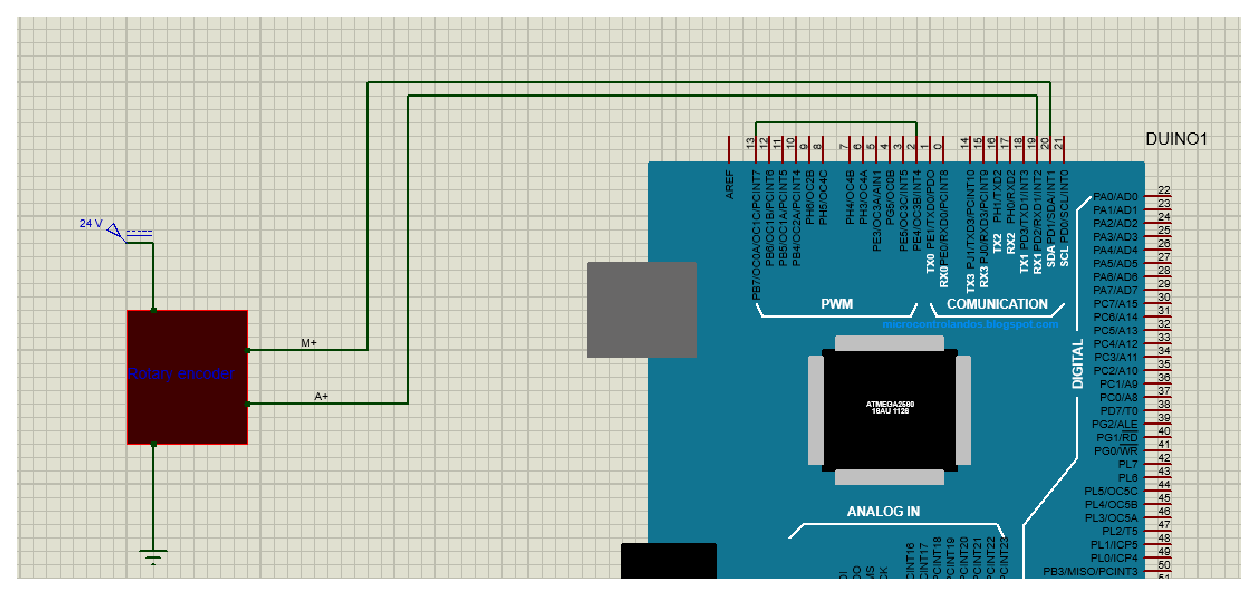
\includegraphics[height=9cm]{bilder/Rot.eps}
\end{center}
\caption{Schaltung des Encoders}
\end{figure}

\subsection{Drucksensor}
\begin{figure}[!htb]
\begin{center}
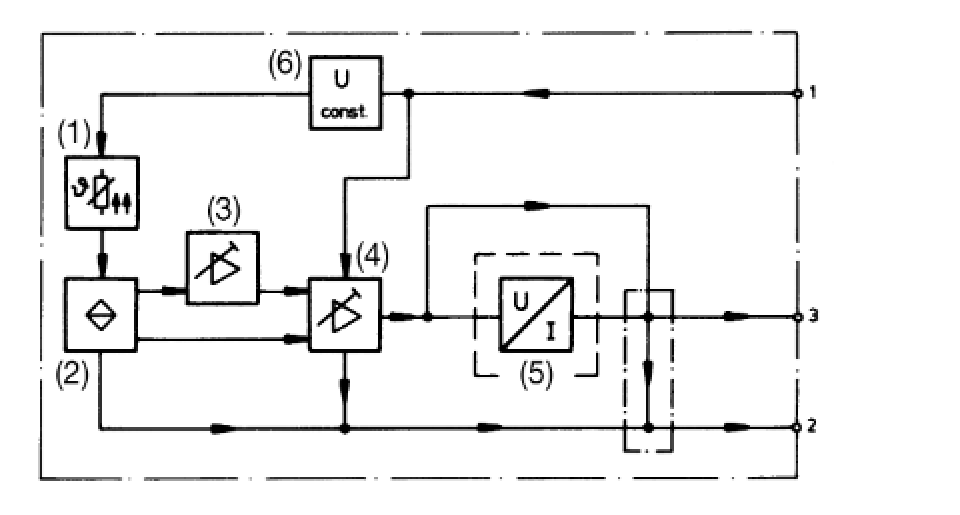
\includegraphics[height=7cm]{bilder/Blo.eps}
\end{center}
\caption{Blockschaltbild[4]}\label{fig:Blo}
\end{figure}


Der Drucksensor funktoiniert indem die druckbelastete Trennmembran 
auf den piezoresistieven Druckmessumformers dr"uckt.

Die  Trennmembran f"uhrt den Druck durch den systematischen Aufbau eines
solchen Drucksensors in Abbildung~\ref{fig:Blo}  
eine Fl"u"ssigkeit der Siliziummembrane mit Widersrandme"ssbr"ucke(2),
die nach dem piezoresistiven Effekt arbeitet und 
"uber eine Temperaturkompensation(1) an eine Konstantspannugsquelle (6)
angeschlo"ssen ist.
Das Ausgang"ssignal der Widerstandsme"ssbr"ucke ist mit
einem Differenzverst"arker mit hohem Eingangswiderstand (4) verst"arkt.
Die Me"ssspanne wird mit Hilfe eines Me"ssspannentrimmers eingestellt.
Eine Nullpunktkorrektur wird vom Verst"arker (3) mit einstellbarer 
Verst"arkung eingestellt. Der Ausgangssignal ist  
 von 0 bis 20 mA .Durch der U/I-Wandler(5) wird 
 das Ausgangssignal in einen angeeigneten Strom umgewandelt. [4]
 
 \begin{figure}[!htb]
\begin{center}
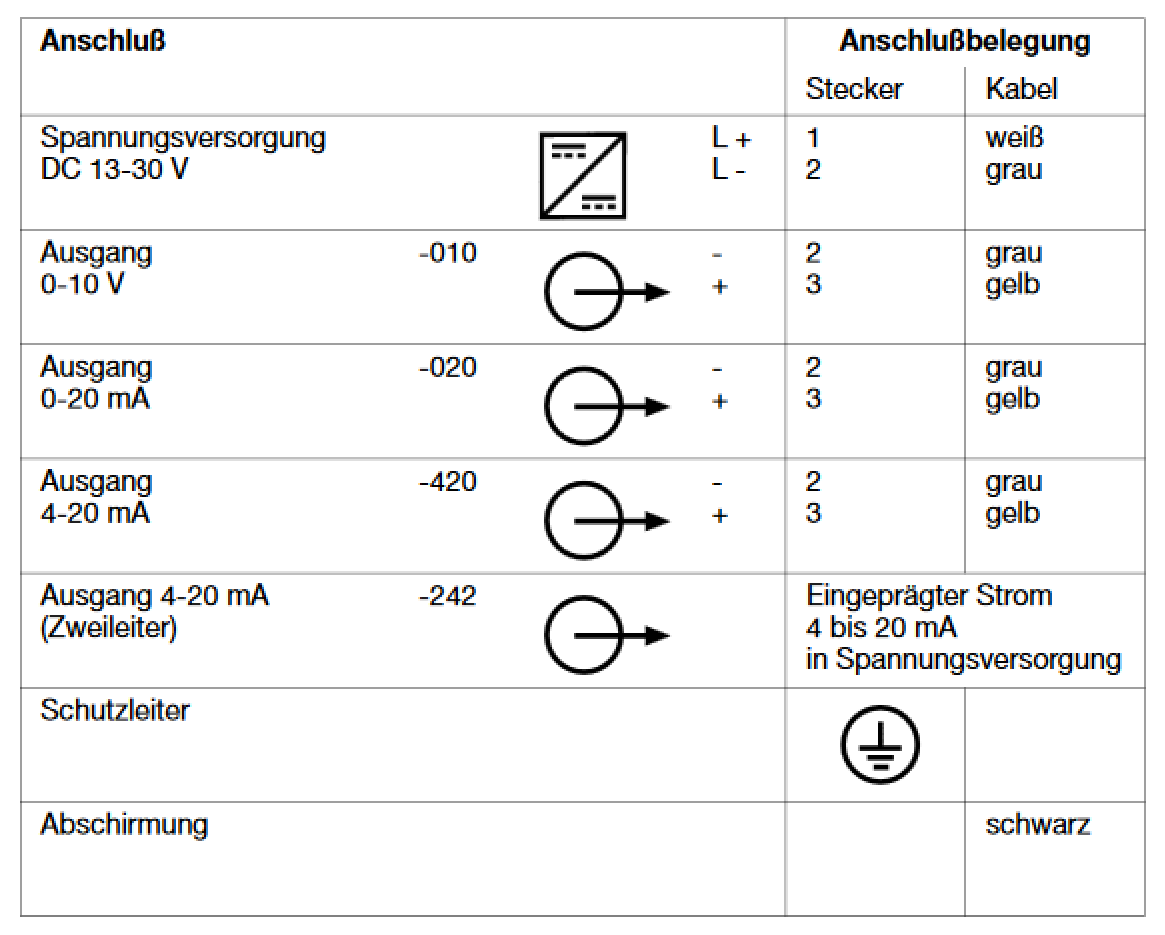
\includegraphics[height=7cm]{bilder/Anschluss.eps}
\end{center}
\caption{Anschlu"ssbelegung[4]}
\end{figure}

Der Referenzdruck ist entweder absolut, 
relativ oder versiegelt. 
  
 Im ge"offneten Raum entspricht der Absolutdruck dem Atmossp"ahrendruck.


Die Differenz zwischen dem absoluten Druck und dem atmosph"arischen ist 
der relative Druck .Der Druck im Beh"alter ist ein bekannter Druck .
Es ist wichtig ,den genauen Referenzdruck zu w"ahlen ,
weil es mehr oder weniger  Fehler eintreten k"onnte[8].

\subsection{PT100 Temperaturf"uhler}

Die maximale Temperatur des Eingriffs und 
die Umgebungstemperatur m"ussen   ber"ucksichtigt werden. 
Die meisten elektronischen Sender des Sensors werden  
nicht richtig funktionieren, 
wenn die Temperatur "uber  107$^\circ$C(225$^\circ$F) l"auft. 
Deswegen ist der Einsatz des entsprechenden Montagezubeh"ors
 zum Beispiel ausreichende L"angen der Impuls, 
 Spulen und so weiter  erforderlich, 
 um  die Sendezelle akzeptable Temperatur der Fl"ussigkeit zu 
 reduzieren. 
 Die Exposition der Elektronik mit Halbleiter der 
 Umgebungstemperaturen hat den Effekt der 
 Besch"adigung von Komponenten. 
 Die meisten elektronischen Bauteile
  k"onnen  nicht  "uber eine Temperatur  
 von 93$^\circ$C(200$^\circ$F)funktionieren  und es gibt eine große Anzahl 
 von Komponenten mit einer maximalen Betriebstemperatur 
 von 85$^\circ$C (185$^\circ$F). 
 Die hohen Temperaturen f"uhren tendenziell
 zu sinkenden elektronischen Energieeffizienz. 
 Auch hier wird empfohlen, 
 die bestm"ogliche K"uhlung des elektronischen Moduls zu gew"ahrleisten.
 Vorstellbar ist auch ein System des Winterschutzes 
 der Elektronik entweder  
 durch Heizdampf, elektrisch oder mittels Thermostat[7].
 
Pt100 ist ein Platin-Widerstand mit einem Nennwiderstand 
von 100$\Omega$ bei einer Temperatur von 0$^\circ$C ,
der in IEC 751 (EN 60751) definiert ist .
Auf Englisch nennt man ihn Resistance Temperature Detector. 
Seit lang werden die Pt100 wie gezeit in Abbildung ~\ref{fig:pt100} in industriellen Unternehmen und 
im Labor benutzt. 
Es gibt auch  andere Pt500 und Pt1000.

\begin{figure}[!htb]
\begin{center}
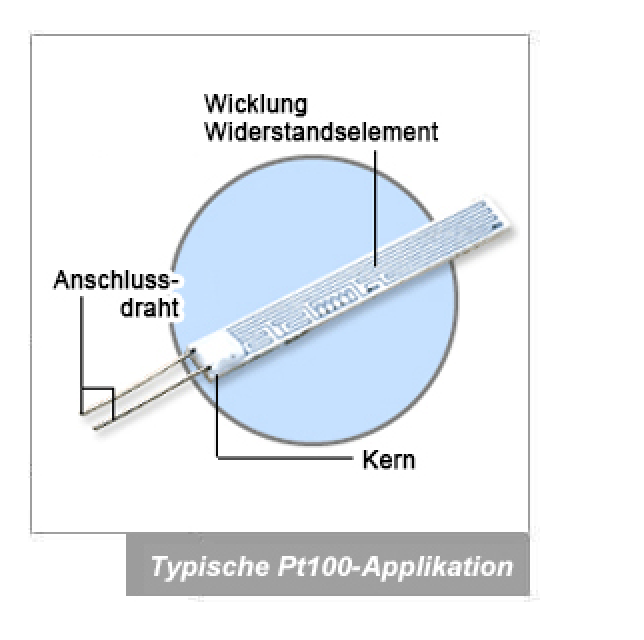
\includegraphics[height=5cm]{bilder/pt100.eps}
\end{center}
\caption{Typische Pt100-Applikation[5]}\label{fig:pt100}
\end{figure}
 
 Pt100 sind stark und nicht empfindlich gegen elektrische St"orungen,
 deshalb sind sie f"ur viele Benutzungen geeignet.
 Außerdem k"onnen die auch in der N"ahe von andere Ger"aten, 
 Motoren und Generatoren gebaut werden, die hohe Spannungen liefern.
 Pt100 haben noch andere Vorteile, die k"onnen große 
 Temperaturbereich von -200$^\circ$C bis 850$^\circ$C messen und lineare sind.
 Außerdem haben die gute Genauigkeit und Austauchbarkeit  
 sowie hohe Stabilit"at f"ur Langzeit[5]. 
 
 \subsection{Bauarten der Pt100}
 
 Alle pt100 sind mit Platin-D"unnschichttechnik produziert, 
 die auf mikrostrukturierten Schichtverbindungen aus Metall, 
 Glas und Keramik basiert. Dar"uber hinaus enthalten die Pt100  
 Sensorelemente aus einer d"unnen Platin-Drahtwicklung, 
 die mit einem Keramik oder Glask"orper verbunden sind.
 Das Element vom Widerstand steckt "ofter in einem Mantelf"uhrer 
 oder einem gleichen sch"utzenden Geh"ause. Auch unter komplizierte 
 Industriebedingungen sind die Pt100 Sensoren stark,
 pr"azise und stabil f"ur lange Zeit.Den Aufbau eines typischen Platin-D"unnschichttechnik
 sehen Sie in Abbildung~\ref{fig:pla}[5].

 
 \begin{figure}[!htb]
\begin{center}
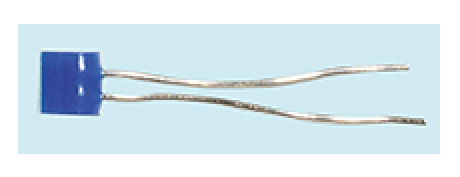
\includegraphics[height=3cm]{bilder/pla.eps}
\end{center}
\caption{Platin-D"unnschichttechnik[5]}\label{fig:pla}
\end{figure}
 
 Um die Widerstandselements zu herstellen, 
 ist es notwendig ein Platin-Material zu nutzen, 
 dessen Widerstand bei unterschiedlichen Temperaturen anerkannt 
 und beschrieben ist. Es gibt eine Widerstands"anderung bei 
 der Temperatur"anderung .Damit die Temperatur aus dem 
 Widerstand abgelesen werden kann,
Eine wichtige Bauart f"ur Pt100  ist der Drahtgewickelte-Widerstand 
wie gezeigt in Abbildung~\ref{fig:dra}. 
Gleichzeitig gibt es zwei Ausstattung  ein mit der Wicklung in einem 
Keramik oder Glasr"ohrchen ,die am meisten verbreitet ist und 
mit der Wicklung außen auf einen Keramik oder Glaskern ,
die mit einer weiteren Glas- oder Keramikschicht  
die f"ur spezielle Umwelteinfl"usse ausgelegt ist[5].

\begin{figure}[!htb]
\begin{center}
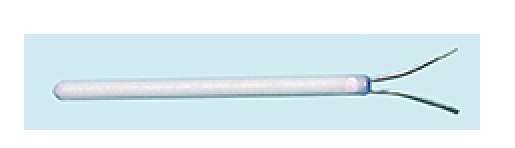
\includegraphics[height=3cm]{bilder/dra.eps}
\end{center}
\caption{Drahtwickelte-Widerstand[5]}\label{fig:dra}
\end{figure}

\subsection{Schaltung der TP100}
\begin{figure}[!htb]
\begin{center}
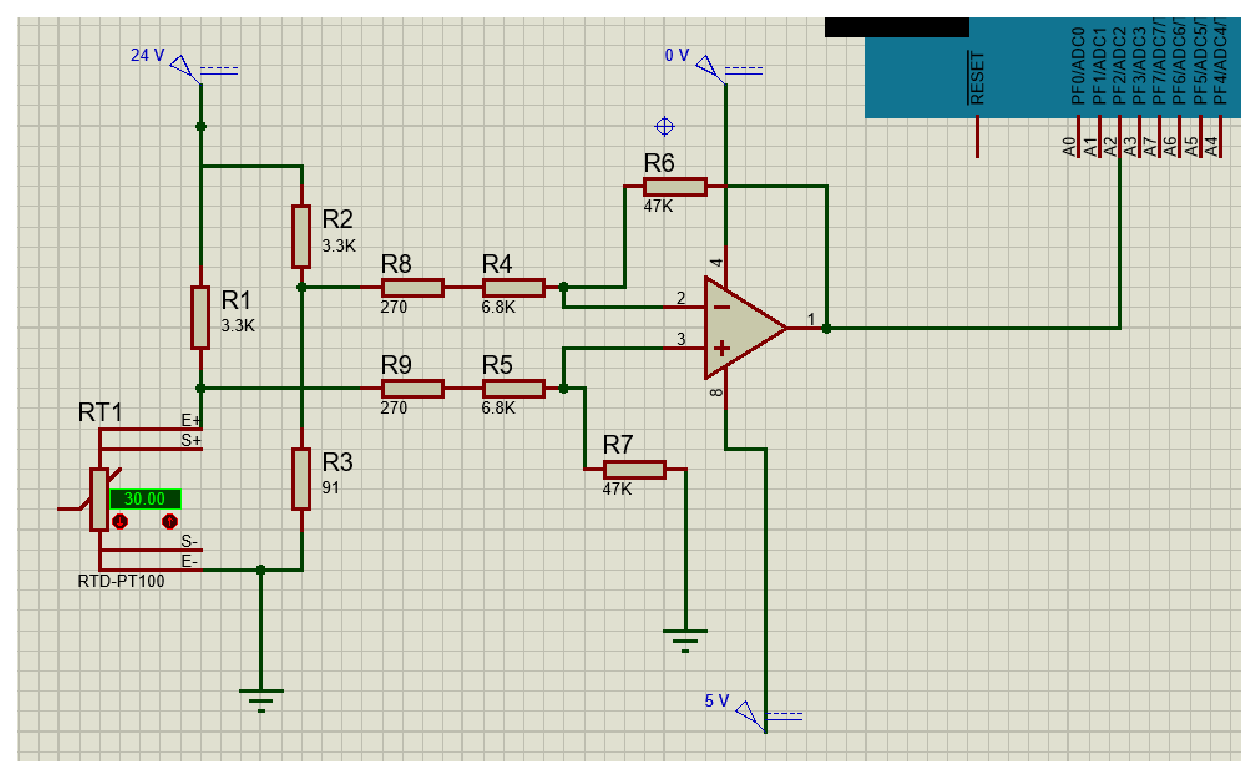
\includegraphics[height=8cm]{bilder/im.eps}
\end{center}
\caption{Schema der Aufbau von TP100}
\end{figure}

\subsection{Dehnmessstreifen}
Ein DMS ist ein Sensor, 
bei dem der Widerstandswert mit der Ausdehnung variiert.
 Die Widerstands"anderung ist auf die minimale Ver"anderung 
 der Linienstruktur im Falle einer Verformung zur"uckzuf"uhren. 
 Wenn der Leiter in L"angsrichtung gestreckt wird, 
 ist die Leiterstruktur d"unner und l"anger, 
 was zu einer gr"oßeren Festigkeit f"uhrt. 
 Diese kleinste Widerstands"anderung gilt als Messwert. 
 Um die Sensibilit"at der DMS zu erh"ohen, 
 sind sie in M"aanderform, was den Leiter als Ganzes verl"angert. 
 In der elektronischen Schaltungstechnik werden Br"uckenschaltungen eingesetzt,
  wenn es darum geht, 
  minimale Schwankungen von Spannung, 
  Strom oder Widerstand zu erkennen. 
  Dies gilt auch f"ur Dehnungsmessstreifen. Um relativ kleine 
  Widerstands"anderungen zu erkennen, werden Dehnungsmessstreifen 
  in Br"uckenschaltungen wie der Wheatstone-Br"ucke angeschlossen und 
  Spannungsdifferenzen in nachgeschalteten Differenzverst"arkern verst"arkt[31].
  
\subsection{DY-Dehnungsmessstreifen}
Die DY-DMS haben zwei parallel angeordnete Messgitter. 
Die typische Anwendung dieser DMS ist die Messung an Biegestangen.Der Aufbau 
eine DY-DMS wird in Abbildung~\ref{fig:DY}gezeigt[26]. 


\begin{figure}[!htb]
\begin{center}
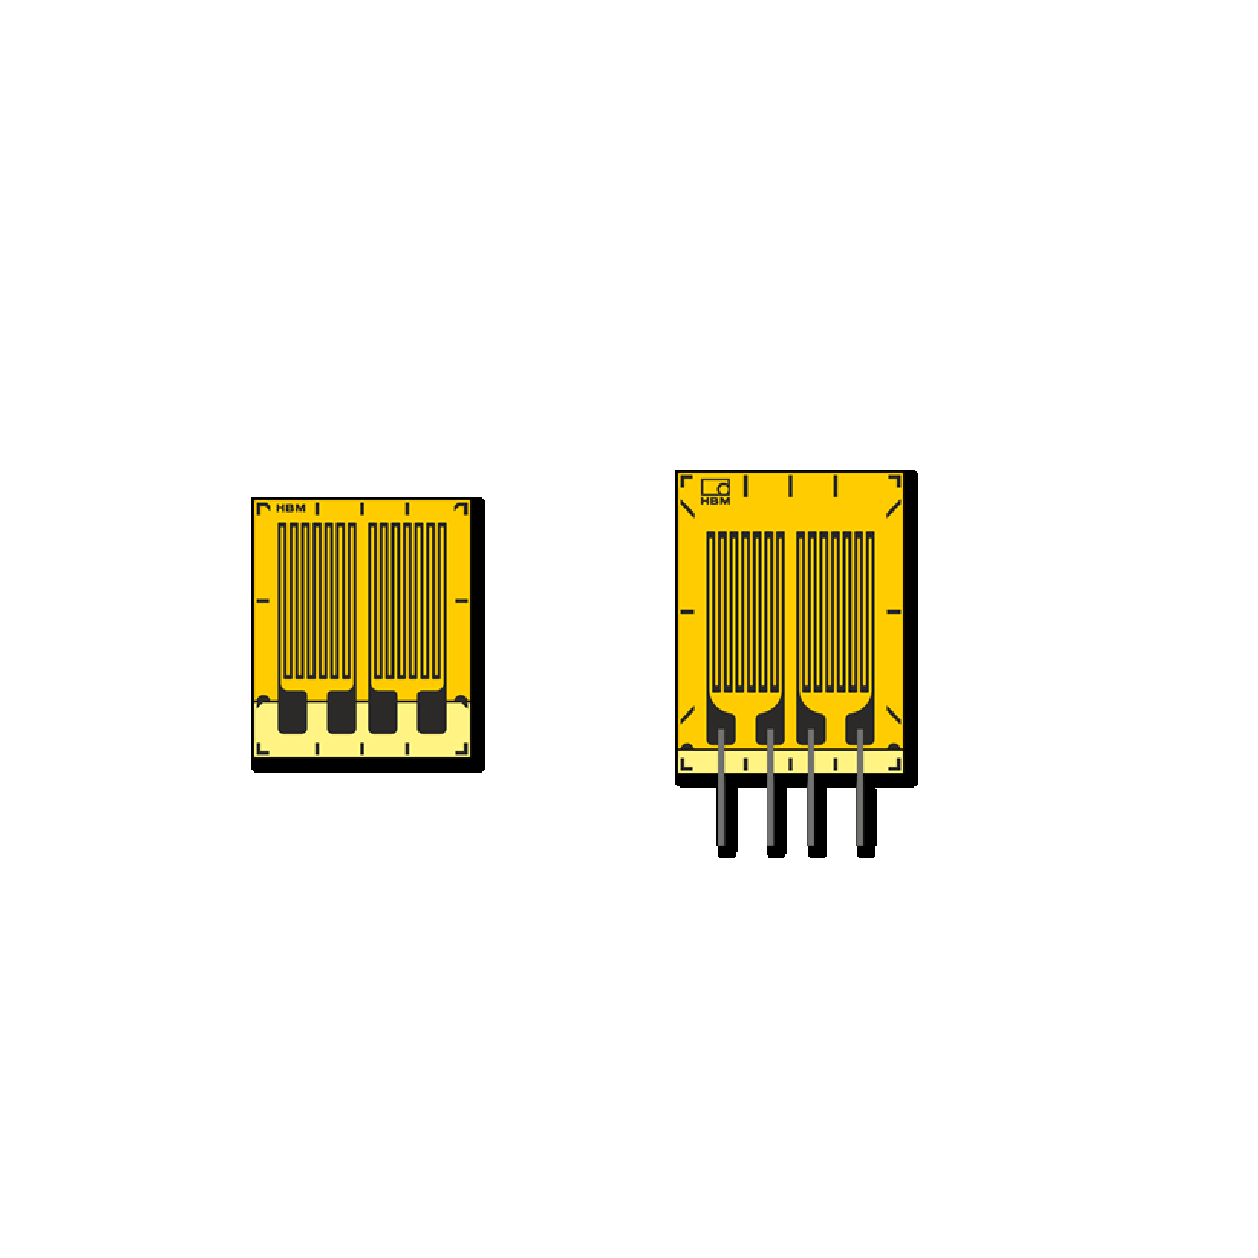
\includegraphics[height=3cm]{bilder/DY.eps}
\end{center}
\caption{DY Doppel-DMS[32]}\label{fig:DY}
\end{figure}


%
\subsection{Elektrische Schaltung der DMS}
Die geringen Widerstandsvariationen eines DMS werden fast ohne 
Ausnahme mit der Wheaststone Br"ucke ermittelt, 
die Abbildung~\ref{fig:w} zeigt die Schaltung: Ub ist eine feste Spannung, 
haupts"achlich eine Gleichspannung, aber es wird auch die Wechselspannung benutzt. 
Dadurch werden unn"otige Thermospannungen entfernt[33].


\begin{figure}[!htb]
\begin{center}
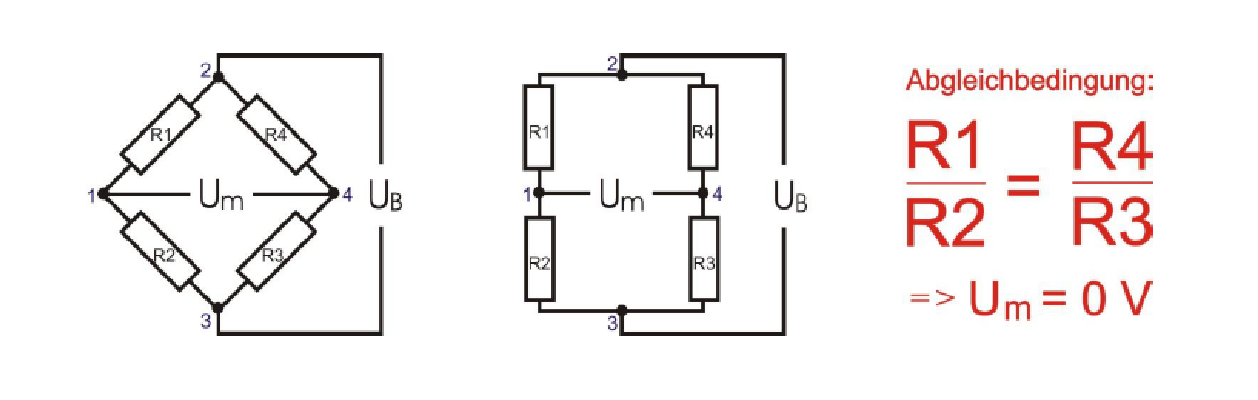
\includegraphics[height=3cm]{bilder/w.eps}
\end{center}
\caption{Wheatestone-Br"ucke mit DMS[33]}\label{fig:w}
\end{figure}





Es ist oft erforderlich, einen negativen Eingang in Arduino zu nehmen. 
 Aber der Arduino nimmt  nur positive Spannungen auf. 
Die unten erkl"arte Methode nimmt die negativen und positiven Werte und 
sendet sie  an Arduino. Die L"osung besteht darin, sowohl den urspr"unglichen 
Eingang als auch einen inversen Eingang zu nehmen und einen mit einem 
Multiplexer auszuw"ahlen. So k"onnen wir den positiven Eingang, wie er ist, 
und den negativen Eingang in umgekehrter Form erhalten. 
Das Signal kann "uber den Ausgang eines Vergleichers bestimmt werden, 
der dem gleichen Eingang wie die Differenzverst"arker ausgesetzt ist.

Die Schaltung besteht aus zwei Differenzverst"arkern. 
Die Schaltung f"ur beide ist genau gleich. 
Aber der angegebene Eingang ist umgekehrt.

(V1-V2 zu einem und V2-V1 zu einem anderen). Man verwendet Operationsverst"arker LM358 ,
 um Differenzverst"arkerteile zu realisieren. 
 Man bekommt zwei Eing"ange, einen umgekehrten und den Original. 
 Wie man dazwischen  w"ahlt, ist im n"achsten Schritt erkl"art. 

Der Vergleich wird benutzt, um das Zeichen des Eingangs 
(negativ oder positiv) zu ermitteln. Eine Komparaturschaltung 
kann mit einem einfachen Operationsverst"arker hergestellt werden. 
Es wird eine positive Feedback gegeben 
(d.h. verbinden Sie die Output mit dem nicht-umkehrenden Anschluss des Operationsverst"arkers) 
mit einem hohen Widerstand. Es wird1Mohm 1K oder 220 Ohm verwendet, 
die auch die Aufgabe erf"ullen sollten. Man schlie"st dem Komparator mit  
zwei Eing"ange (V1 und V2) an. V2 auf nicht invertierende Anschluss und 
V1 auf invertierende Anschluss. Der Komparator gibt den Ausgang Null aus, 
wenn der V2-V1<0 und Vcc wenn der V2-V1>0 ist, und der Ausgang des Komparators wird auch 
als Eingang des Multiplexers (CD4053) verwendet.

Wir haben Jetzt  drei Leitungen :einen tats"achlichen Eingang, 
sein invertiertes Gegenteil und das Vorzeichen des Eingangs. 
Diese drei k"onnen direkt an den Multiplexer verbunden werden und der 
richtige Eingang kann im Code ausgew"ahlt werden (digitalRead() der Vorzeicheneingang) 
oder wenn die Erhaltung eines Pins von Bedeutung ist, 
kann CD4053 mux benutzt werden. Die Schaltug wird in 
die Abbildung~\ref{fig:Dehn}  gezeigt[34].

\begin{figure}[!htb]
\begin{center}
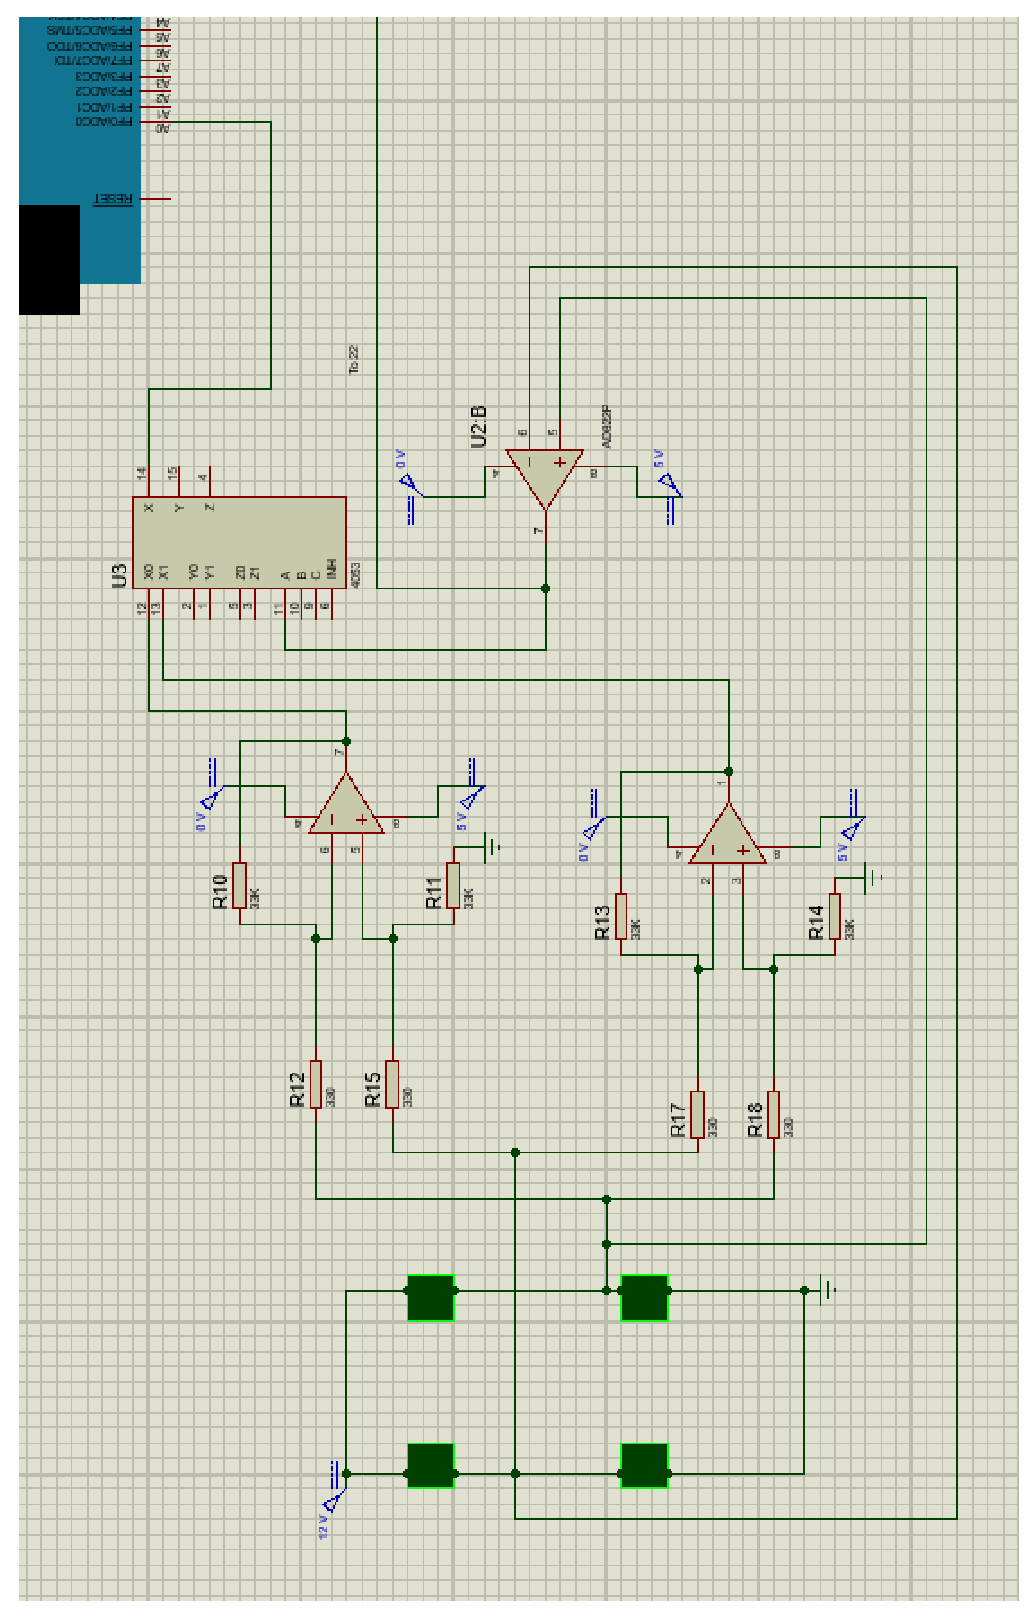
\includegraphics[height=7cm]{bilder/Dehn.eps}
\end{center}
\caption{Schaltung der Dehnmessstreifen}\label{fig:Dehn}
\end{figure}








\subsection{Carnot-Prozess}

Der Carnot-Prozess ist daher ein Modell f"ur zirkul"are Prozesse, 
weil er Energie sehr effizient umsetzt, was er sehr gut kann, 
weil er absolut reversibel funktioniert, mit dem Vorteil, 
dass durch den Carnot-Prozess keine Entropie entsteht. 
Der Nachteil ist, dass es nur in der Theorie funktioniert, 
nicht in der Realit"at. Der Name ist der Carnot-Prozess, 
weil er von dem Franzosen Sadi Carnot erfunden wurde, 
der sich der Effizienzverbesserung von Dampfmaschinen widmete 
und der als sehr inoffiziell bezeichnet wird, 
f"ur den seine wissenschaftlichen Forschungen oft 
wichtiger sind als seine Umgebung[35]. 

Damit dieser zyklische Prozess reversibel ist, 
werden die folgenden Zustands"anderungen ber"ucksichtigt, 
die das Arbeitsmedium st"andig aufsetzt:  \newline
1$\rightarrow$2:  isotherme W"armeaufnahme: Die W"arme"ubertragung erfolgt 
mit unbegrenzten kleinen Temperaturunterschied. 
Die Entropie nimmt zu, aber es findet keine Entropie statt.\newline

2$\rightarrow$3:   Isentrope Expansion: Das Arbeitsmedium-Volumen steigt,
 Druck- und Temperatur sinken.Das l"auft adiabat, das bedeutet ohne W"armestrom,
  ohne Reibung und ohne Energieverlust. \newline
  
3$\rightarrow$4: Isotherme W"armeabgabe: Hier auch erfolgt die W"arme"ubertragung
 mit unbegrenzt kleinen Temperaturunterschieden, so dass nur die Entropie 
 das System verl"asst, die sowieso mit der W"arme zu tun hat, 
 aber es entsteht keine Entropie. \newline
 
4$\rightarrow$1: Isentrope Kompression: Das Arbeitsfluid wird komprimiert,
 dadurch werden Druck und Temperatur erh"oht. 
 Dies geschieht auch adiabasisch und ohne Energieverlust[35]. \newline
 
 Die vier Zustandswechsel haben die Gemeinsamkeit, 
 dass sie nur dann wie dargestellt ablaufen k"onnen, 
 wenn sie unbegrenzt langsam sind und die Maschine unbeschr"ankt gro"s ist. 
 Isotherme Zustands"anderungen treten bei unbegrenzten kleinen 
 Temperaturunterschieden  auf. Damit W"arme verdr"angt werden kann, 
 ist es notwendig, entweder unendlich lange zu warten oder 
 eine unendlich gro"se Fl"ache f"ur die W"arme"ubertragung zur Verf"ugung zu 
 stellen. Und wenn man versucht, isentrope Zustands"anderungen zu 
 erreichen, dann stellt man recht schnell fest, dass man unbegrenzt 
 langsamer arbeiten muss, so dass keine Entropie entsteht[35]. 

 Die Abbildung~\ref{fig:pv} zeigt ,wie man den Carnot-Prozess in einem p,v- Diagramme anzeigen kann.
 \begin{figure}[!htb]
\begin{center}
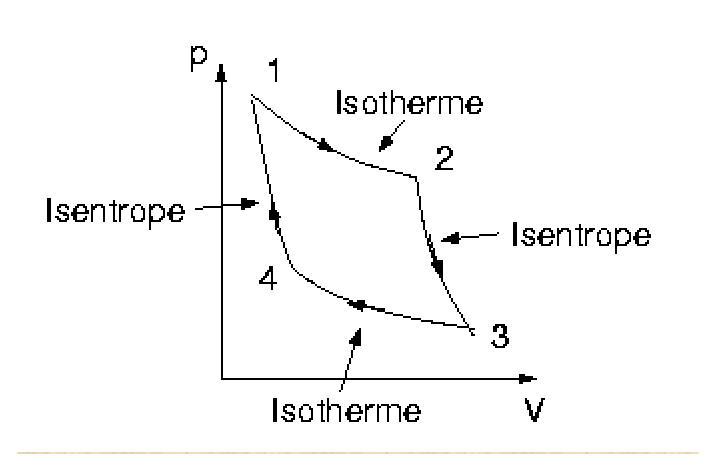
\includegraphics[height=9cm]{bilder/pv.eps}
\end{center}
\caption{PV Diagramm[36]}\label{fig:pv}
\end{figure}





%



 









\section{Industrie 4.0}
%
\subsection{Allgemein}

Industrie 4.0 ist ein Schlagwort, das die vierte industrielle 
Revolution beschreibt. Durch die Vernetzung der Maschine mit 
den Produkten wurde die traditionelle Produktionshierarchie abgebaut. 
Dezentrale Selbstorganisation ersetzt die zentrale Steuerung. 
Die Produkte werden aktiv in den Produktionsprozess eingebunden. 
Ressourcen- und Energieeinsparung ist eine Voraussetzung 
f"ur die Prozessplanung und erfolgreiche Produktion.
 Es werden so genannte intelligente Fabriken aufgebaut.
Der Name wurde zum ersten Mal auf der Hannover Messe 2011 verwendet[9]. 
In Deutschland sind die Empfehlungen zur Umsetzung des Arbeitskreises 
Industrie 4.0 an die Bundesregierung weitergeleitet worden.
 Auf der Hannover Messe 2013 wurde ein Endbericht der Arbeitsgruppe
  eingereicht und parallel dazu nahm die von den drei Fachverb"anden 
  Bitkom, VDMA und ZVEI gegr"undete Industrieplattform 4.0 
  ihre Arbeit auf. Ziel ist es, die Aktivit"aten 
  in diesem Feld in Zukunft zu koordinieren[10].
Mechatronische Systeme,Cyberphysikalische Systeme und das "Internet der 
Dinge" oder "Internet der Dienste" sind technologische 
Voraussetzungen[11]. 





\subsection{Voraussetzung der Technik}
%
\subsubsection{Mechatronische Systeme}
Mechatronische Systeme bestehen aus einem Basissystem.
Sensoren, Aktoren und ein Informationssystem.
Transformation. Die Umsetzung der
das mechatronische System, in dem es betrieben wird.
Das Basissystem ist in der Regel ein
mechanisch, elektromechanisch, hydraulisch oder pneumatisch.
Generell ist jedoch jedes physikalische System als Basissystem denkbar, 
d.h. mechatronische Systeme mit einer bestimmten 
hierarchischen Struktur k"onnen abgebildet werden[12].
Die Abbildung~\ref{fig:me} zeigt ein Beispiel eines 
mechatronischen System.

\begin{figure}[!htb]
\begin{center}
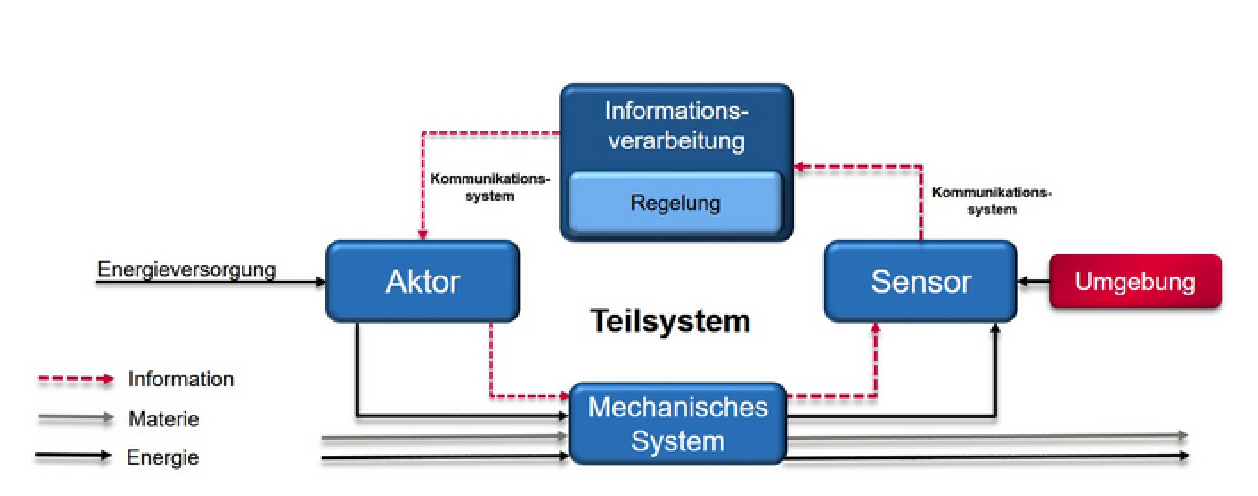
\includegraphics[height=5cm]{bilder/me.eps}
\end{center}
\caption{Mechatroniches System[12]}\label{fig:me}
\end{figure}



\subsubsection{Die Bedeutung Cyper Physical Systems}

 CPS sind mechanische Komponenten 
durch intelligente Netzwerke und Informationstechnologien miteinander verkn"upft.
 Sie erlauben die Steuerung und "uberwachung komplexer Systeme und Infrastrukturen.
 Cyber-physikalische Systeme spielen in Industrie 4.0 eine wichtige Rolle.
 Sie sind moderne mechanische Komponenten, 
 Software und Informationstechnologie. Die Vernetzung der verschiedenen 
 Komponenten "uber Netzwerke wie das Internet erm"oglicht die Steuerung, 
 Regelung und "uberwachung komplexer Infrastrukturen. 
 Der Informationsaustausch zwischen Objekten und vernetzten 
 Systemen kann in Echtzeit, drahtlos oder drahtgebunden erfolgen. 
 Die Komponenten cyber-physikalischer Systeme umfassen sowohl
  mobile Ger"ate als auch station"are Maschinen, Systeme und Roboter. 
  Cyber-physikalische Systeme spielen in Industrie 4.0 eine wichtige 
  Rolle. Die technologischen Grundlagen des CPS werden durch 
  Naturwissenschaften wie Informatik, Mathematik, Maschinenbau, 
  Elektrotechnik und Robotik geliefert[13].\newline
  Das Betriebsprinzip ist auf vernetzte Sensoren, 
  Aktoren und Software aufgebaut. 
  Sensoren ermitteln Messdaten aus der physikalischen Welt 
  und "ubertragen sie "uber Netzwerke an die Software, die sie verarbeitet. 
  Daraus resultieren die Regeldaten, die die Software "uber 
  das Netzwerk an die Stellglieder "ubermittelt. 
  Cyberphysikalische Systeme sind in Abbildung~\ref{fig:cps} aufgebaut 
  und zeichnen sich durch einen hohen Grad 
  an Komplexit"at aus und werden beispielsweise f"ur den Aufbau von Smart Power Grids, 
  modernen Produktionsanlagen oder in der Medizintechnik eingesetzt.
  Viele verschiedene Komponenten und Technologien werden ben"otigt, 
  damit cyberphysikalische Systeme ihre Aufgaben erfüllen können.
   Dazu gehören Zum Beispiel:
 \begin{itemize}
   \item Sensoren
    \item Aktoren 
     \item eingebettete Systeme
      \item Netzwerkinfrastrukturen [14]
    \end{itemize}
   
  
  
  
 %





    
    
 \subsubsection{Erkl"arung des Begriffs Das Internet der Dinge}
 
 Der Begriff Internet der Dinge wie gezeigt in Abbildung~\ref{fig:F} erkl"art,
  dass der Computer zunehmend wie
   ein Ger"at verloren geht und durch intelligente Objekte 
   zu ersetzen ist.Um im Interesse der Menschen zu sein, 
   sollte das Internet der Dinge die Menschen bei 
   ihren Aktivit"aten unbemerkt st"arken. 
   Kleinere eingebetteten Computer sind so konstruiert, 
   dass sie Menschen helfen, ohne abzulenken oder Aufmerksamkeit zu ablenken. 
   
  Das Internet der Dinge beschreibt die Verbindung von klar 
   identifizierbaren physischen Objekten mit einer virtuellen 
   Darstellung in einer internetgleichen Struktur. 
   Sie besteht nicht mehr nur aus menschlichen Beteiligten, 
   sondern auch aus Dingen[15].
 
 
 \begin{figure}[!htb]
\begin{center}
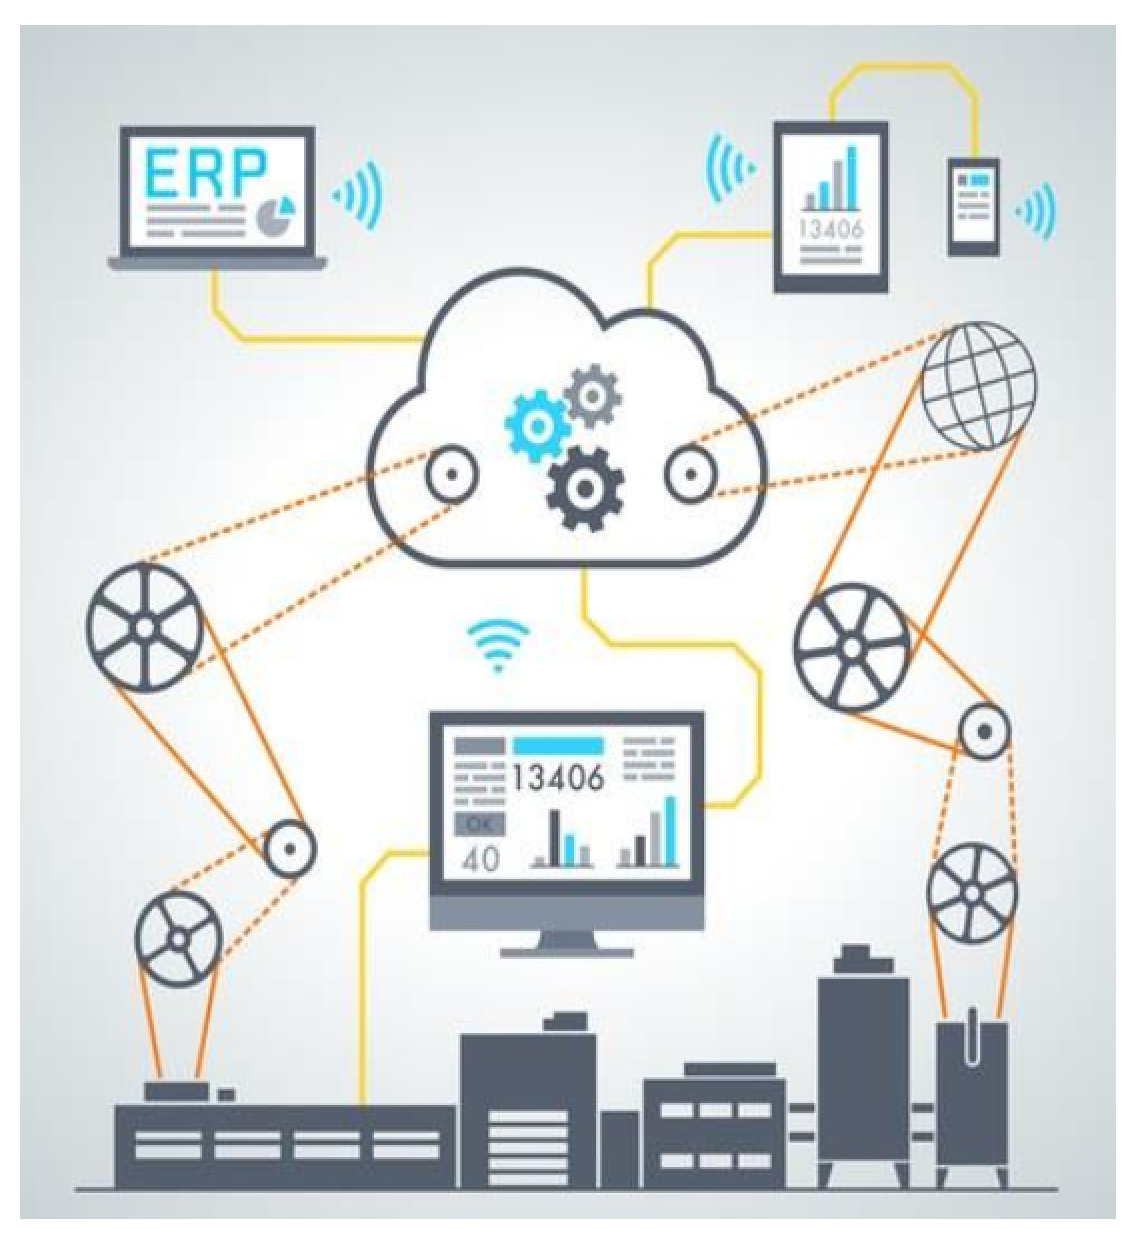
\includegraphics[height=8cm]{bilder/F.eps}
\end{center}
\caption{Internet der Dinge[16]}\label{fig:F}
\end{figure}

Die automatische Identifikation durch RFID wird oft als Basis 
f"ur das Internet der Dinge betrachtet. 
Objekte k"onnen aber auch mittels Barcode oder 
2D-Code eindeutig identifiziert werden. 
Ger"ate wie Sensoren und Aktoren erm"oglichen
 die Erweiterung der Funktionalit"at, 
 indem sie Zust"ande erfassen oder Aktionen durchf"uhren.
  Das Internet der Dinge erm"oglicht es, 
  reale Informationen effektiv zu erfassen und digital 
  zu verarbeiten, unter den technischen Bedingungen und Anforderungen, 
  die oft als notwendig betrachtet werden, 
  um die Medienl"ucke zwischen der realen und 
  der virtuellen Welt zu reduzieren. 
  Die Internetsichten der Objekte werden 
  in die Produktionsumgebung "ubertragen. 
  Die Industrie wird in der Lage sein, 
  sehr stark individualisierte Produkte in kleinen Mengen 
  (bis zu einer einzigen Menge) herzustellen, 
  und zwar bei hoher Ressourcenproduktivit"at 
  und entsprechender Geschwindigkeit[17].







 






\section{Hardware}
Drahtlose Ad-hoc oder Sensornetzwerke erm"oglichen 
die Verbindung von Netzwerken zwischen zwei oder mehreren Endger"aten. 
Die Ger"ate verbinden sich ohne feste Infrastruktur. Dies f"uhrt dazu, 
dass f"ur die Kommunikation keine festen Routingknoten 
bestehend aus Datenspeicher, Sensoren, Stromquelle und 
Funkmodul ben"otigt werden. Dar"uber hinaus haben sie mehrere 
Optionen f"ur den Aufbau eines Sensorknotens und die Entwicklung, 
um von mehreren Anwendungen zu profitieren.    
Zu Beginn der 70er Jahre wurden die ersten AD-Hoc-Netze vom US-Milit"ar 
entwickelt und werden heute noch im zivilen Bereich verwendet. 
Um einen drahtlosen Sensor in Arduino zu optimieren, 
m"ussen die Hardwarekomponenten getestet werden. 
Im weiteren Verlauf des Prozesses werden 
einige Versionen von Arduino dargestellt.[18]

\subsection{Die Versionen von Arduino}

Arduino ist eine Open-Source-Elektronikplattform, 
die auf einfach zu bedienender Hard- und Software aufbaut. 
Arduino-Karten sind in der Lage, die Eing"ange -
 das Licht eines Sensors, 
 einen Finger auf einer Taste oder eine Twitter-Mitteilung 
 zu lesen und zu einem Ausgang zu machen,um einen Motor zu schalten, 
 eine LED einzuschalten, 
 etwas online zu ver"offentlichen. 
 Sie k"onnen ihrer Karte mitteilen, was sie tun soll, 
 indem Sie eine Reihe von Befehlen an den Mikrocontroller 
 auf der Karte senden. 
 Dazu wird die Programmiersprache Arduino 
 (basierend auf Verkabelung)benutzt und die Arduino-Software (IDE)  
  auf die Verarbeitung basiert[19].
Im Laufe der Jahre war Arduino der Kopf hinter Tausenden von Projekten, 
von Alltagsgegenst"anden bis hin zu komplizierten wi"senschaftlichen
Instrumenten. Eine internationale Gemeinschaft von Studenten, 
Amateuren, K"unstlern, Programmierern und Profis haben sich um diese 
Open-Source-Plattform angesiedelt, ihre Beitr"age haben 
zu einer unglaublichen Menge an zug"anglichem Wissen gef"uhrt, 
das f"ur Anf"angern und Experten eine gro"se Hilfe sein kann.

Arduino wurde am Ivrea Interaction Design Institute als 
leichtes Werkzeug f"ur Rapid Prototypen f"ur Studenten ohne Elektronik
 und Programmierausbildung entwickelt[20]. 
 Als die Arduino-Karte eine breitere "Offentlichkeit erreichte, 
 begann sie sich an neue Anforderungen und Probleme anzupassen 
 und unterscheidet ihr Angebot von einfachen 8-Bit-Karten 
 "uber Produkte f"ur IoT-Anwendungen, Laptops, 3D-Druck und 
 integrierte Umgebungen. Alle Arduino-Karten sind komplett 
 Open Source, so da"s die Benutzer sie selbstst"andig entwickeln 
 und an ihre spezifischen Bed"urfnisse anpassen k"onnen. 
 Die Software ist auch Open Source, 
 und sie wird mit den Beitr"agen von Anwendern 
 auf der ganzen Welt gewachsen..[21]

\subsection{ATmega328 Boards}
\subsubsection{Definition}

Der ATmega328 ist ein von Atmel entwickelter Ein-Chip-Mikrocontroller 
aus der megaAVR-Familie (sp"ater wurde Atmel von Microchip Technology 
im Jahr 2016 "ubernommen). Es verf"ugt "uber einen modifizierten 
8-Bit-RISC-Prozessorkern mit Harvard-Architektur.
Ab 2013 wird der ATmega328 h"aufig in vielen Projekten und autonomen 
Systemen eingesetzt, in denen ein einfacher, 
stromsparender und kosteng"unstiger Mikrocontroller ben"otigt wird. 
Die wahrscheinlich h"aufigste Implementierung dieses Chips ist die 
beliebte Arduino-Entwicklungsplattform, n"amlich die Modelle Arduino 
Uno und Arduino Nano[22].

\subsubsection{Eigenschaften}
Der Atmel 8-Bit-AVR-RISC-basierte Mikrocontroller kombiniert 
32-kB-ISP-Flash-Speicher mit Lese- und Schreibfunktionen, 
1-kB-EEPROM, 2-kB-SRAM, 23 Allzweck-E / A-Leitungen, 32 
Allzweck-Arbeitsregister, drei flexible Timer / Z"ahler mit 
Vergleichsmodi, internen und externen Interrupts, seriell 
programmierbarem USART, einer byteorientierten seriellen 
2-Draht-Schnittstelle, seriellem SPI-Port, 6-Kanal-10-Bit-A / D-Wandler 
(8 Kan"ale in TQFP- und QFN / MLF-Paketen) , programmierbarer Watchdog-Timer mit 
internem Oszillator und f"unf per Software w"ahlbaren Energiesparmodi. 
Das Ger"at arbeitet zwischen 1,8 und 5,5 Volt. Das Ger"at erreicht 
einen Durchsatz von ann"ahernd 1 MIPS pro MHz[23].




\subsection{Arduino Uno}

In der Abbildung~\ref{fig:Uno} ist ein Arduino Uno,der ein Mikrocontroller-Board auf Basis des ATmega328P ist. 
Es besitzt 14 digitale Ein-/Ausgangspins 
(einschlie"slich 6 PWM-Ausg"ange), 6 analoge Eing"ange, 
einen 16 MHz Quarz, einen USB-Anschluss, eine Steckdose, 
einen ICSP-Anschluss und eine Reset-Taste. Es enth"alt alles, 
was man braucht, um den Mikrocontroller zu unterst"utzen; 
der wird einfach "uber ein USB-Kabel an einen Computer 
angeschlossen oder der wird  mit einem AC/DC-Adapter oder einer 
Batterie eingeschaltet, um  ihn zu starten. Man kann an UNO arbeiten, 
ohne  Sorgen zu machen, etwas falsch zu machen, 


 Uno bedeutet eins auf Italienisch und wurde anl"asslich 
 der Ver"offentlichung von Arduino Software (IDE) 1.0 ausgew"ahlt. 
 Die Uno-Karte und die Arduino-Software Version 1.0 (IDE)
 waren die Referenzversionen von Arduino, 
 die sich nun zu neuen Versionen weiterentwickelt haben. 
 Die Uno-Karte ist die erste aus einer Reihe von Arduino USB-Karten 
 und das Referenzmodell f"ur die Arduino-Plattform; eine komplette 
 Liste der derzeitigen, vergangenen und veralteten Karten findet man 
 im Arduino-Kartenverzeichnis [21].
\begin{figure}[!htb]
\begin{center}
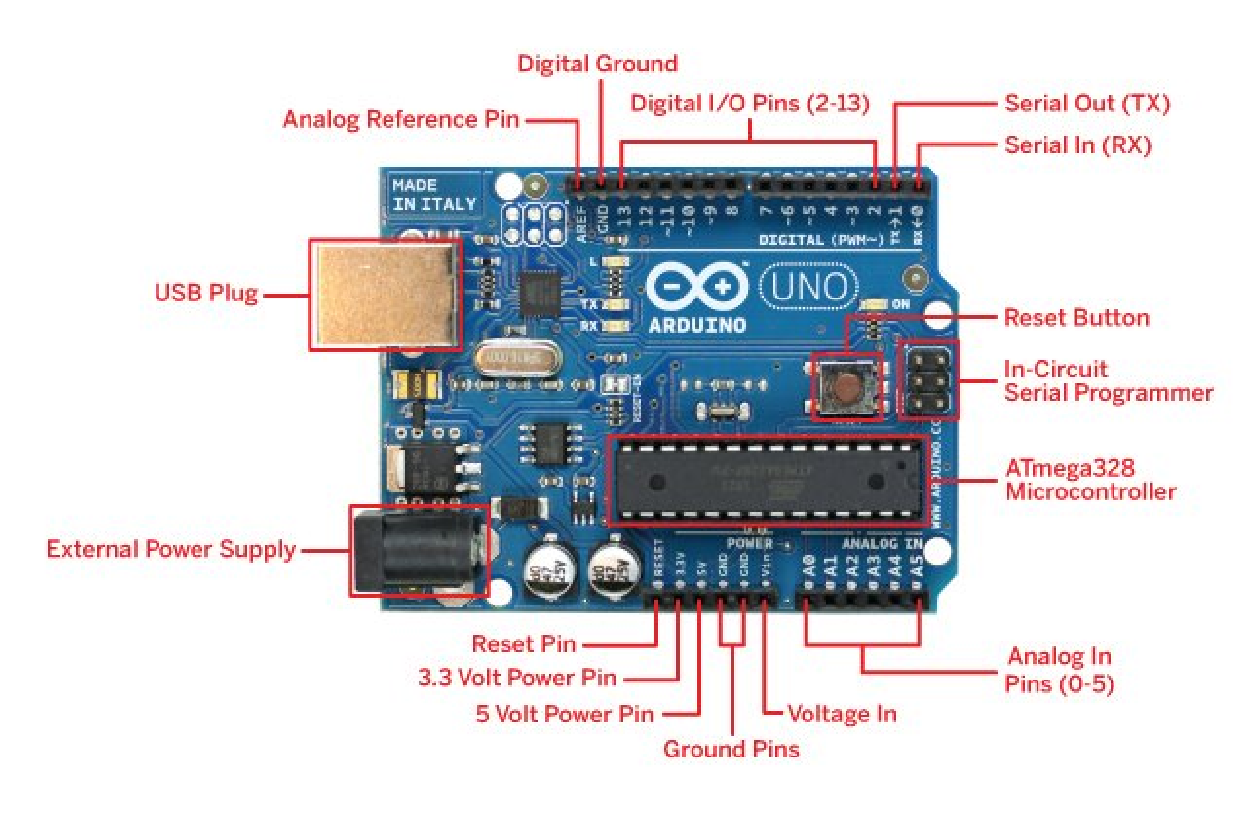
\includegraphics[height=7cm]{bilder/Uno.eps}
\end{center}
\caption{Arduino Uno (eigene Darstellung)}\label{fig:Uno}
\end{figure}



\subsection{ATmega2560}
\subsubsection{Definition}

Das Arduino Mega 2560 ist ein Mikrocontroller-Board, das auf dem 
ATmega2560 basiert. Es verf"ugt "uber 54 digitale Eingangs- / Ausgangspins 
(von denen 14 als PWM-Ausg"ange verwendet werden k"onnen), 16 analoge Eing"ange,
 4 UARTs (serielle Hardware-Ports), einen 16-MHz-Quarzoszillator, 
 einen USB-Anschluss, eine Netzbuchse, einen ICSP-Header und 
 eine Reset-Taste. Es enth"alt alles, was zur Unterst"utzung des 
 Mikrocontrollers ben"otigt wird. Schlie"sen Sie es einfach mit 
 einem USB-Kabel an einen Computer an, oder versorgen Sie es mit 
 einem Netzteil oder Akku, um loszulegen. Das Mega ist kompatibel mit 
 den meisten Schilden, die f"ur den Arduino Duemilanove 
 oder Diecimila entwickelt wurden[24].

\subsubsection{Eigenschaften}
Der RISC AVR-basierte 8-Bit-Microchip-Mikrocontroller 
verbindet 256KB ISP-Flash-Speicher, 8KB SRAM, 4KB EEPROM, 
86 gemeinsame I/O-Leitungen, 32 allgemeine Arbeitsregister, 
Echtzeitz"ahler, 6 flexible Betriebsstundenz"ahler mit Vergleichsmodis, 
PWM, 4 USART, 2 Byte serielle 2-Draht-Schnittstelle, 
16-Bit-A/D-Wandler und JTAG-Schnittstelle f"ur chipbasiertes Debugging. 
Das Ger"at schafft einen Durchsatz von 16 MIPS bei 16 MHz und 
funktioniert zwischen 4,5 und 5,5 Volt.
Durch die Ausf"uhrung leistungsf"ahiger Befehle 
in einem einzigen Taktzyklus erreicht das Ger"at einen 
Durchsatz von etwa 1 MIPS pro MHz, 
der den Stromverbrauch und 
die Verarbeitungsgeschwindigkeit ausgleicht[24].

\subsection{Arduino Mega2560}
Arduino Mega 2560 wie beschrieben in Abbildung~\ref{fig:Mega} ist eine Mikrocontroller-Karte auf 
Basis des ATMega2560 mit 54 
digitalen I/O-Pins (davon 14 als PWM-Ausg"ange nutzbar), 
16 analogen Eing"angen, 4 UARTs (serielle Hardwareschnittstellen), 
einem 16 MHz Quarzoszillator, 
einer USB-Schnittstelle, einem Leistungsstecker, 
einem ICSP-Header und einem Reset-Taster. Es enth"alt alles, 
was man braucht, um den Mikrocontroller zu unterst"utzen. 
Man schlie"st die Karte einfach "uber USB an einen Computer an oder man 
schlie"st sie mit einem DC/AC-Adapter oder einer Batterie an, 
um sie zu starten. Arduino Mega ist mit den meisten der 
f"ur Arduino Duo, Duemilanove oder 
Diecimila entwickelten Schilde kompatibel[21].

\begin{figure}[!htb]
\begin{center}
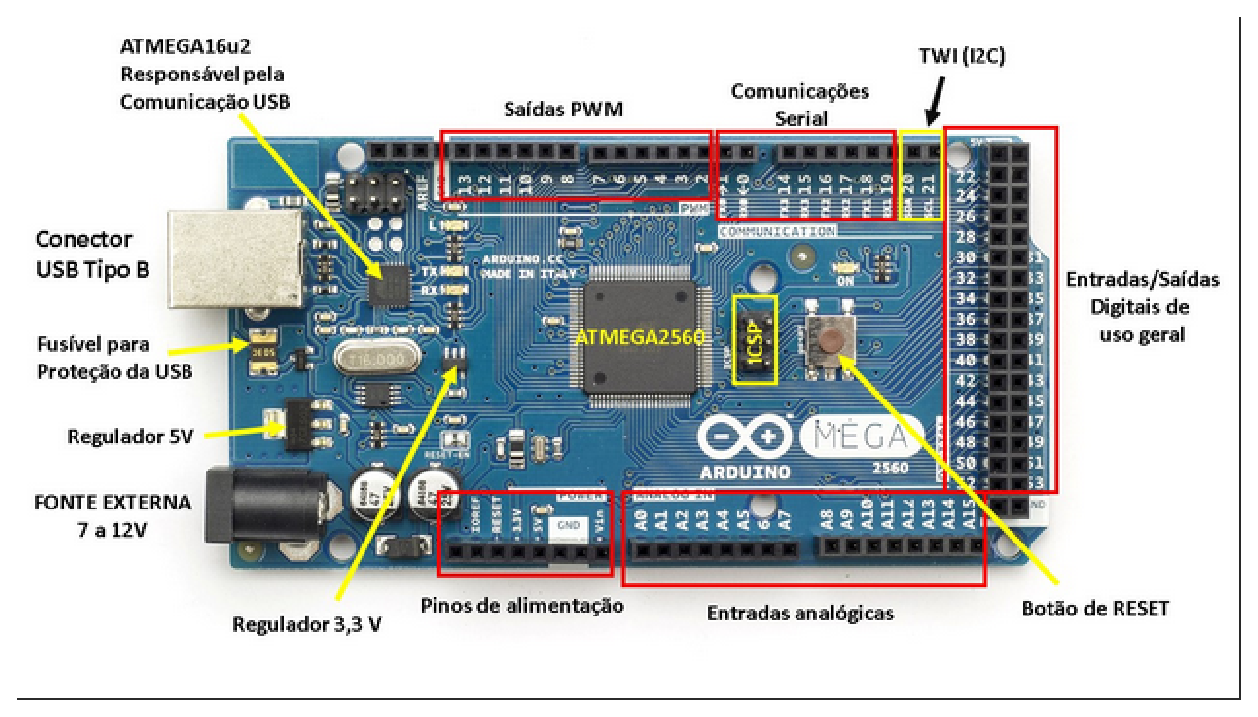
\includegraphics[height=7cm]{bilder/Mega.eps}
\end{center}
\caption{Arduino Mega 2560 Eigene Abbildung in Anlehnung mit[21]}\label{fig:Mega}
\end{figure}
















\section{PHP}
\subsection{Bedeutung PHP}

PHP ist eine Open-Source-Skriptsprache 
f"ur den allgemeinen Gebrauch, 
die speziell f"ur die Webprogrammierung entwickelt wurde 
und in HTML integriert werden kann. 
 PHP zeichnet sich von clientseitigen Sprachen
  wie Javascript dadurch aus, 
  dass der Code auf dem Server ausgef"uhrt wird, 
  wo er eine HTML-Ausgabe erzeugt, 
  die an den Kunde geschickt wird. 
  Der Kunde bekommt daher nur das Ergebnis der Skriptausf"uhrung, 
  ohne wissen zu k"onnen, wie der tats"achliche Code aussieht. 
  Es besteht  die M"oglichkeit, 
  dass Ihr Webserver alle Ihre HTML-Dateien mit PHP pr"uft, 
  weil es dann wirklich nichts gibt, 
  was man dem Benutzer sagen kann, was es in petto enth"alt.

Das Besondere an der Benutzung von PHP ist, 
dass es f"ur Anf"anger extrem einfach zu bedienen ist,
 aber auch eine Vielzahl von Funktionen f"ur den 
 professionellen Programmierer bietet.  
 Die lange Liste der PHP-Funktionen zu lesen,macht kein Problem.
 Weil es m"oglich ist,
 in weniger Stunden einfache Skripten zu erstellen[25].

\subsection{Hauptgebiete der PHP-Skripte}

Es gibt drei Hauptbereiche, in denen PHP-Skripte verwendet werden :
\begin{itemize}
\item Serverseitige Programmierung. 
Dies ist die traditionelle und das wichtigste Bereich 
von PHP. Es braucht drei Dinge,
 um es zu benutzen: 
 Der PHP-Parser (CGI\footnote{CGI bedeutet allgemein Verwaltungsrechner Schnittstelle} oder Servermodul), 
 ein Webserver und ein Webbrowser. Es muss einen Webserver 
 ausgef"uhrt werden, der mit einer PHP-Installation verbunden ist. 
 Es ist m"oglich, auf die Ergebnisse des PHP-Programms 
 "uber einen Webbrowser zu reagieren, 
 der die Seite "uber den Server anzeigt. 
 Es kann all dieses Skript auf Ihrem PC ausgef"uhrt werden, 
 wenn man zuerst mit der PHP-Programmierung ausprobieren will.
 
 
\item Befehlszeilenprogrammierung. 
Es ist ebenfalls m"oglich, PHP-Skripte zu schreiben, 
die ohne Server oder Browser funktionieren. 
Alles, was es ben"otigt ist, ist der PHP-Parser. 
Die Nutzungsart ist ideal f"ur Programme, 
die h"aufig mit cron (unter Linux) oder (unter Windows) 
durchgef"uhrt werden. 
Skripte k"onnen auch f"ur 
eine einfache Textverarbeitung verwendet werden.



\item Schreiben von Desktop-Applikationen. 
PHP ist wahrscheinlich nicht die allerbeste Sprache, 
um Desktop-Anwendungen mit grafischer Oberfl"ache zu schreiben, 
aber wenn Sie PHP sehr gut kennen und einige weiterf"uhrende 
PHP-Features in Ihren clientseitigen Applikationen nutzen m"ochten, 
k"onnen Sie PHP-GTK nutzen, um derartige Programme zu schreiben. 
Auf diese Art haben Sie auch die M"oglichkeit, 
plattform"ubergreifende Applikationen zu schreiben. 
PHP-GTK\footnote{GTK bedeutet in dieser Arbeit ein Paket von Sprachverbindungen f"ur PHP} ist eine Erweiterung von PHP, 
die in der Hauptdistribution nicht enthalten ist.
\end{itemize}

PHP kann auf allen wichtigen Betriebssystemen genutzt werden, 
einschließlich Linux, 
vielen Unix-Varianten (einschlie"slich HP-UX, Solaris und OpenBSD), 
Microsoft Windows, MacOS, RISC OS und möglicherweise anderen. 
PHP ist auch kompatibel mit den meisten aktuellsten Webservern. 
Dazu gehören Apache, Microsoft Internet Information Server, 
Personal Web Server, Netscape und iPlanet Server, 
Oreilly Website Pro Server, Caudium, Xitami, 
OmniHTTPd und viele andere. 
F"ur die meisten Server stellt PHP ein eigenes Modul zur Verf"ugung, 
f"ur andere, die den CGI-Standard erf"ullen, 
kann PHP als CGI-Prozessor eingesetzt werden[26]. 
%
\subsection{Warum PHP?}

PHP ist die am h"aufigsten verwendete Programmiersprache und die Sprache 
f"ur die Entwicklung dynamischer Webanwendungen,
weil es einfach funktioniert.
Die PHP-Programmierung kann alles tun, 
was eine andere Programmiersprache 
f"ur dynamische Anwendungen tun kann.
Der Vergleich von Programmiersprachen ist schwierig, 
da jede ihre Vor- und Nachteile hat. Grunds"atzlich ist 
jedoch die Aussage, dass PHP einfach und schnell ist. 
Die Nachteile von PHP sind erh"ohrter Netzwerktraffic,
Gerschwindigkeitsnachteil beim Kompilieren des Skriptes[38].
Experten zufolge ist die Syntax von PHP der von ASP 
 und JSP "uberlegen und leistungsf"ahiger als ColdFusion und viel 
einfacher zu erlernen als Pearl. Diese Vorteile machen PHP 
zur am weitesten verbreiteten Programmiersprache[27].

\subsection{Datenbank}

Die effiziente Speicherung und Abfrage gro"ser Datenmengen hat wesentlich 
zum Erfolg des Internets beigetragen, das in der Regel 
mit Hilfe von Datenbanken realisiert wird: Seiten wie Yahoo, Amazon 
und Ebay sind stark von der Zuverl"assigkeit von Datenbanken abh"angig, 
in denen gro"se Mengen an Informationen gespeichert sind.
Der Datenbank-Support ist jedoch nicht im Web, 
f"ur den Webentwickler reserviert, verschiedene leistungsstarke 
Implementierungen werden zu relativ niedrigen Preisen 
(oder sogar kostenlos) angeboten, 
das Hinzuf"ugen von Such- und Sortierfunktionen auf Ihrer 
Website ist viel einfacher, und die Steuerung von Berechtigungen 
ist dank der Berechtigungskontrollfunktionen 
vieler Datenbanksysteme einfach[28].

\subsection{Definition von SQL}

SQL k"onnte kurz als Standardsprache f"ur die Interaktion mit 
relationalen Datenbanken beschrieben werden. 
SQL ist aber keine Computersprache wie C, C++ oder PHP. 
Es ist vielmehr ein Interface-Tool, 
mit dem man verschiedene Befehle ausf"uhren kann. 
SQL ist jedoch nicht nur eine Abfragesprache (wie der Name schon sagt), 
sondern bietet eine Vielzahl von Werkzeugen f"ur die Datenbankinteraktion:

\begin{itemize}
\item Datenstrukturdefinition: SQL kann die verschiedenen Konstruktionen 
definieren, die die Datenbank zum Speichern von Daten verwendet.
\item Datenabfrage: SQL kann Daten aus einer Datenbank abrufen 
und in einem einfach zu lesenden Format anzeigen.
\item Datenbearbeitung: SQL kann Daten einf"ugen, 
aktualisieren und aus der Datenbank l"oschen.
\item Datenzugriffskontrolle: SQL kann verwendet werden, um zu steuern,
 wer Daten basierend auf dem Benutzer anzeigen, einf"ugen, 
 aktualisieren und l"oschen darf.
 \item Datenintegrit"at: SQL verhindert Datenverluste aufgrund paralleler 
 Datenaktualisierungen oder Systemausf"alle[28].
 



Nach der Definition ist SQL besonders f"ur relationale Datenbanken bestimmt. 
Eine analytische Datenbank ist eine Datenbankimplementierung, 
bei der alle Daten in Tabellen mit einem einzigartigen Namen 
untergliedert sind. Es kann eine Tabelle in Form von Datenwerten wie beschrieben in Abbildung~\ref{fig:Daten}
aufgebaut werden, bei der die Position der Daten pro Zeile/Spalte 
definiert wird. Dieses Format wird in der Regel 
auch f"ur die Darstellung verwendet[28].
 

 \end{itemize}
 \begin{figure}[!htb]
\begin{center}
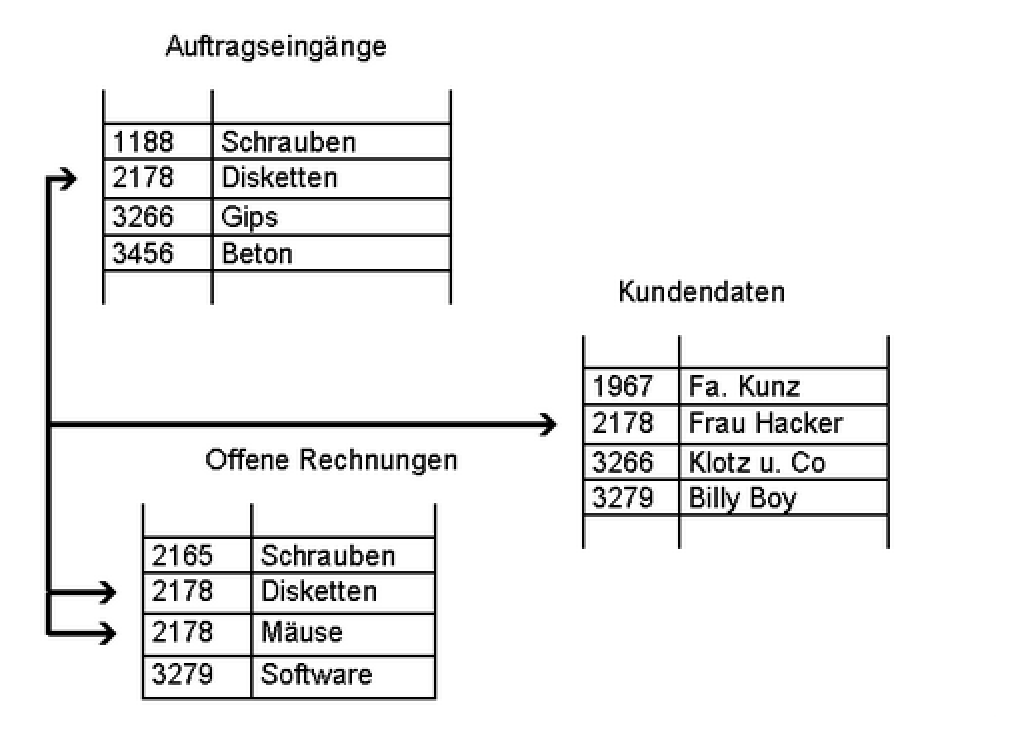
\includegraphics[height=6cm]{bilder/Daten.eps}
\end{center}
\caption{Beispiel einer relationalen Datenbank[29]}\label{fig:Daten}
\end{figure}




\subsection{was ist MySQL?}

MySQL ist ein zuverl"assiger SQL-Datenbank-Server, 
der von T.c.X DataKonsultAB in Stockholm, Schweden, entwickelt wurde[30]. 
Seit der Entwicklung im Jahr 1995 hat sich MySQL zu einem der 
beliebtesten Datenbankserver der Welt etabliert. 
Diese Akzeptanz ist zum Teil auf die Schnelligkeit, 
Stabilit"at und Flexibilit"at der Lizenzpolitik von MySQL zur"uckzuf"uhren, 
die im Vergleich zu PHP aufgrund ihrer Funktionen und vieler 
vordefinierter und einfach zu bedienender Schnittstellenfunktionen 
eindeutig die beliebteste Datenbank geworden ist[28].
MySQL organisiert, stellt dar, bewahrt und modifiziert 
Daten der klassischen Aufgabe 
eines Datenbank-Managementsystems.
Es arbeitet als Client-Server-System: Die entsprechende Datenbank ist der Server.
 Die clientseitige Software sendet Befehle an die Datenbank. 
 Die Datenbank wandelt die Auftr"age in vollziehbaren Code um, 
 f"uhrt die Auftr"age aus und schickt die Informationen "uber sie an den Kunden[28][30].
 
\subsection{Serielle Communication}

Die Universal Asynchronous Transmitter Software Library (UART) wird 
f"ur die RS232-basierte serielle Kommunikation zwischen zwei 
elektronischen Geräten verwendet. Bei der seriellen Kommunikation werden 
nur zwei Kabel ben"otigt, um Daten in beide Richtungen zu "ubertragen. 
Die Daten werden im seriellen Format an den Logikpin1, auch bekannt als Mark, 
gesendet. Die Daten"ubertragung beginnt, wenn dieser Pin auf Logik 0,
 auch bekannt als SPACE, wechselt. Das letzte gesendete Bit ist das 
 Stopp bit mit Logik 1. Serielle Daten werden in der Regel als 10-Bit-Frame gesendet, 
 der sich aus einem Startbit, 8 Daba-Bits und einem Stoppbit und keinem Priorit"atsbit zusammensetzt.
Die Abbildung~\ref{fig:AS} zeigt, wie das Zeichen A "uber die serielle Kommunikation 
gesendet werden kann. Zeichen A hat das Bin"armodell ASCII 01000001,
 wie in der Abbildung dargestellt, das Startbit wird zuerst gesendet, 
 gefolgt von 8 Datenbits 01000001, und schließlich wird das Stoppbit  gesendet.




\begin{figure}[!htb]
\begin{center}
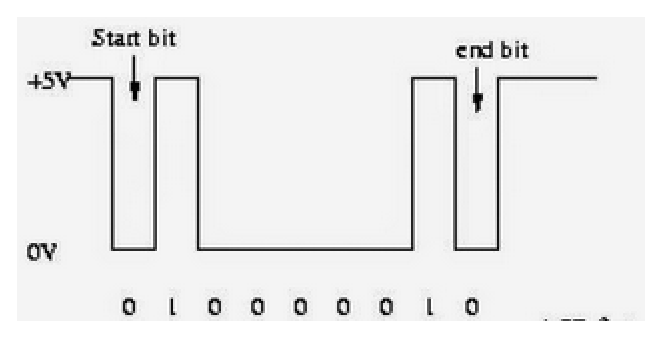
\includegraphics[height=6cm]{bilder/AS.eps}
\end{center}
\caption{Sendung der Character A in Serial Communication[40]}\label{fig:AS}
\end{figure}



Die Bit-Timings sind bei der seriellen Kommunikation sehr wichtig, 
und der Sender (TX) und der Empf"anger (RX) m"ussen die gleichen Bit-Timings 
haben. Das Bit-Timing wird durch die Baudrate gemessen, die die Anzahl 
der "ubertragenen oder empfangenen Baudraten pro Sekunde angibt. 
Typische Baudraten sind 4800,9600,19200,19200,38400 usw. 
Beispielsweise werden bei einem Betrieb mit 9600 Baudrate mit einer 
Bildgr"o"se von 10 Bit pro Sekunde 960 Zeichen gesendet oder empfangen. 
Das Timing zwischen den Bits betr"agt dann etwa 104ms[40]. 

















\section{Softwarepaket}

die Allgemeine Idee ist die Industrialisierung eines Kompressores im 
Industrie 4.0.Die Sensoren liefern die Werten und diese Werten m"ussen 
von Arduino zu dem PC gelesen und geliefert.Um die Graphe zu erstellen,
wird PHP benutzt. Danach wird die Integrale berechnet.
Es wird auch SQL verwendet ,um die Daten zu speichern.

\subsection{Sensoren Auslesen}

Es werden im Programm Arduino alle Eing"ange den Sensoren und Variable defeniert.
Es wird 3 PT100 benutzt und jeder liefert 5 Werten f"ur 5 Cyclus das bedeutet 15 Werten. 
Drucksensor liefert 100 Werten bzw 500 Werten f"ur 5 Cyclus sowie den Dehnmessstreifen.
Aus diesem Grund wird es den Durschnitswert gemacht, um insgesamt 
203 werten zu bekommen.Die drei Interrupt die definiert sind, Signal A, Signal M und S.
Die Interruput S wird gemacht, weil man 5 Umdrehungen braucht. Signal 13 ist als Output definiert und schickt das Signal zu den Pin S,
damit diese Interruption funktionieren kann. Nachdem die Informationen bekommen wurden , m"ussen  diese Interuptionen deaktiviert werden.



\subsection{Sendung der Daten}

Um die Daten zu senden, es wird drei wichtigen Funktionen ben"otigt.Diese Funktionen sind Serial Beginn,
Serial Println und Baudrate.Die Funktion Serial Beginn() weist 
den Arduino an, eine serielle Verbindung mit 9600 bps herzustellen.
Mit der funktion Serial Println wurde die serielle Verbindung gesendet 
und pr"uft ,ob die daten von 3 Sensore der Temperature,Druck und Dehnmesstsreifen in PHP gezeigt werden .
Die Funktion Buadrate hat die gleiche Aufgabe wie Serial Beginn(). die geh"ort zu PHP 
und sie ist sehr wichtig , damit die Komminication zwischen PHP und Arduino richtig gemacht wird.
   
\subsection{Empfang der Daten}

Bei der Empfang der Daten sollte der serielle Port vom Arduino definiert werden. 
Danach wurde es ein Objekt Serielle erzeugt,damit der Empang der Daten gemacht wird.
Die fonction deviceOpen spielt eine wichtige Rolle, um die Daten zu empfangen.
Ohne diese Function k"onnte keine Kommunication angefangen werden. Da f"angt die
RX zu leuchten und das bedeutet der Start der Kommunication mit Arduino.
Bevor PHP eine Nachricht zu Arduino schickt ,ist es notwendig in diesem Fall eine Wartzeit zu machen, Weil PHP eine Wartezeit 
ben"otigt, um die Daten zu lesen, denn Arduino braucht Zeit , um die Werten zu schicken.
Die Werten, die von PHP gelesen werden sind 203 Werten ,3werten von 
den Temperatursensoren ,100 Werten von Drucksensoren und 100 Werten von Dehnmessstreifen.
Diese Werten werden im Serielle Communication gespeichert und dann werden
 diese Werten Zeileweise gelesen,daf"ur wird die Funktion ReadMessageByLine verwendet.
Die Werten werden danach als Ergebnis in einem Tabelle gespeicht werden.
Nach dem alle Werten gelesen sind, schlie"st die Funktion deviceopen den seriellen Port,d.h die Kommunication ist abgeschlossen.


\subsection{Verarbeitung der Daten in PHP}

Im programm PHP werden die Werten von Temperatursensoren,Drucksensor und 
Dehnmessstreifen umgewandelt. Bei den Temperatursensoren müssen die Temperatuspannungen umgewandelt,
damit man an Ende die Werten in Celisius bekommt.Dafür müssen die Widerstände der Temperatursensoren berechnet werden.
Um die zu berechnen , wird diese Gleichung benutzt:

\begin{equation}\label{eq:paran}
 Rt = av + b
\end{equation}
 F"ur die Berechnung der Wert A wird diese Gleichung benutzt:
 
\begin{equation}\label{eq:paran}
 a = \frac{Rmax-Rmin}{Vsmax-Vsmin}
\end{equation}

B ist der minimale Widerstand und es wird die Wert 91bei V=0 benutzt.
Danach werden Vsmax und Vsmin berechnet.

\begin{equation}\label{eq:paran}
 Vsmax = Vb(+) - Vb(-)
\end{equation}

\begin{equation}\label{eq:paran}
 Vb(+) = V\frac{Rt}{Rt+R} =24 \frac{200}{200+3300} = 1,37 V
\end{equation}

\begin{equation}\label{eq:paran}
 Vb(-) = V\frac{Rt}{Rt+R} =24 \frac{91}{91+3300} = 0,64 V
\end{equation}

\begin{equation}\label{eq:paran}
 Vsmax = Vb(+) - Vb(-) =1,37 -0,64= 0,73 V
\end{equation}

Nach der Berechnung wurde es festgestellt dass die Werte von Vsmax zu klein ist. 
Aus diesem Grund muss ein Operationelverstärker benutzt werden.
Laut der Gleichung der Operationelverstärker wird Vsmax neu berechnet mit dieser Formel wie folgt.

\begin{equation}\label{eq:paran}
 Vsmax = \frac{R7}{R8+R4}(Vb(+)-Vb(-)) =\frac{47000}{270+6800}(0,73) = 4,85 V
\end{equation}


\begin{equation}\label{eq:paran}
 Vsmin =  Vb(+) - Vb(-)
\end{equation}

\begin{equation}\label{eq:paran}
 Vb(+) = V\frac{Rt}{Rt+R} =24\frac{91}{91+3300}=0,64
\end{equation}


\begin{equation}\label{eq:paran}
 Vb(-) = V\frac{Rt}{Rt+R} =24\frac{91}{91+3300}=0,64
\end{equation}

laut der Berechnung Vsmin=0 und schlie"st sind alle Werten Berechnet ,um die Wert von a zu bekommen 

\begin{equation}\label{eq:paran}
a = \frac{200-91}{4,85} =22,47
\end{equation}
Wenn die Rt berechnet ist, k"onnte die Temperatur zu Celisius laut dieser Formelsatz umgewandelt werden.

\begin{equation}\label{eq:paran}
T = \frac{Rt -R0}{R0.\alpha}
\end{equation}

Bei der Drucksensor wurde es  auch ein Paar Berechnungen gemacht um die 
Werten zu Konvertieren.Damit der Graph(P,V) erstellt werden k"onnte. 
Der Drucksensor ist linear ,deshalb wird die Methode der Dreisatz gemacht ,um den Ausgangsstrom zu Bar konvertieren.
\begin{equation}\label{eq:paran}
Druck\underline{\ }Voltage = \frac{Druck\underline{\ }Ergebnis}{1023}.5
\end{equation}

Laut der folgenden Gleicheung wird der Strom berechnet.
\begin{equation}\label{eq:paran}
U = R.I 
\end{equation}
Wenn der Strom berechnet ist ,musste zu bar umgewandelt sein. Der Drucksensor funktioniert im Bereich [0,16],
deshalb wird die wert 16 bei der Umwandlung genutzt.
\begin{equation}\label{eq:paran}
Konvertiertdruck =\frac{Druck\underline{\ }I*16}{20*10^{-3}}
\end{equation}

Die Werten der DMS m"ussen auch konvertiert werden. Mit den konvertierten 
Werten konnte das Diagramm der Moment erstellt werden.
In diesem Fall werden noch \(\epsilon \), \(\sigma \) und der Moment berechnet werden.

\begin{equation}\label{eq:paran}
DMS\underline{\ }Voltage = \frac{DMS\underline{\ }Ergebnis}{1023}.5
\end{equation}

\begin{equation}\label{eq:paran}
\epsilon  = \frac{DMS\underline{\ }Voltage}{K.DMS\underline{\ }Vs.100}
\end{equation}

\begin{equation}\label{eq:paran}
\sigma  = E*\epsilon
\end{equation}


\begin{equation}\label{eq:paran}
Moment = \frac{\sigma*10^9*DMS\underline{\ }Igz}{DMS\underline{\ }Ymax}
\end{equation}


Der Berechnete Moment ist die Konvertierte Werte der DMS und mit diesen Werten ,könnte das Graph erstellt werden.
Alle diese Berechnungen werden in PHP gemacht, weil Arduino nicht in der Lage ist, alle diese Berechnungen zu machen.

Die Abbildung~\ref{fig:Orga} zeigt das Organigramm, das die Arbeit von PHP erkl"art

\begin{figure}[!htb]
\begin{center}
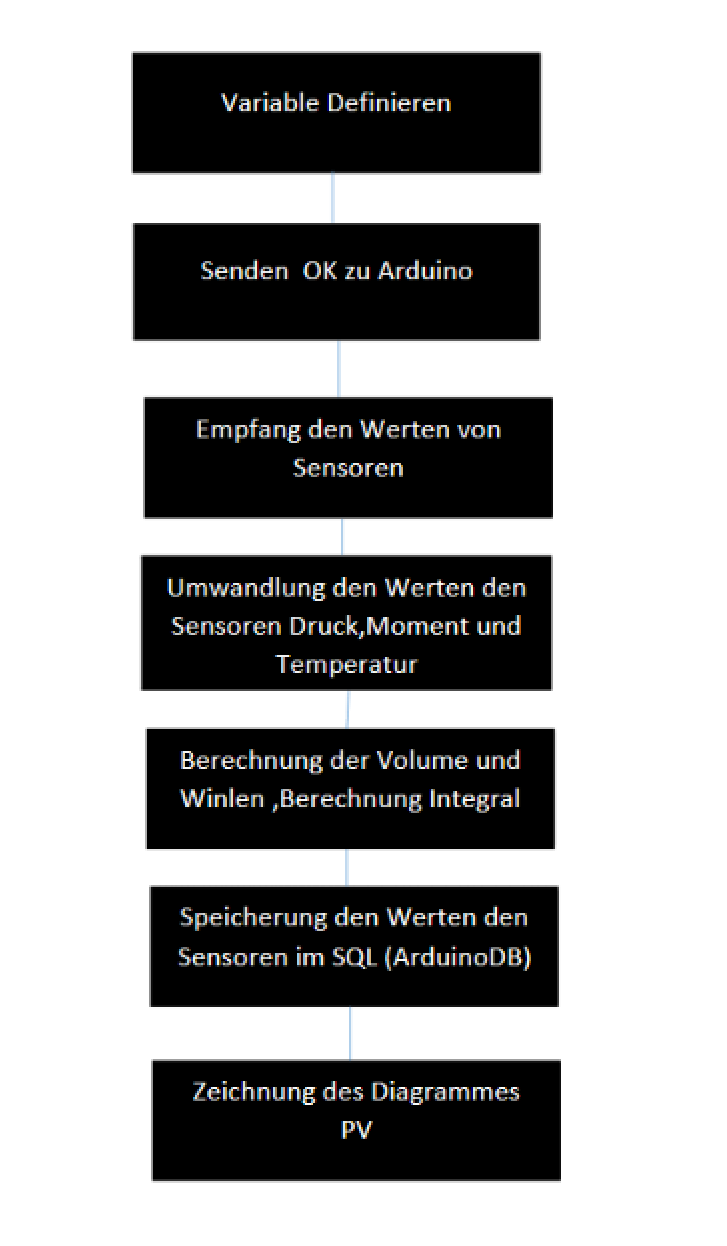
\includegraphics[height=20cm]{bilder/Orga.eps}
\end{center}
\caption{Organigramm PHP}\label{fig:Orga}
\end{figure}


\begin{figure}[!htb]
\begin{center}
\includegraphics[height=25cm]{bilder/or.eps}
\end{center}
\caption{Organigramm Arduino}\label{fig:Orga}
\end{figure}












%\appendix
\addcontentsline{toc}{section}{Abbildungsverzeichnis}
\listoffigures
\addcontentsline{toc}{section}{Tabellenverzeichnis}
\listoftables
% Abk"urzungsverzeichnis
\addcontentsline{toc}{section}{Abk"urzungsverzeichnis}
\section*{Abk"urzungsverzeichnis}
\begin{acronym}
\acro{IOT}{Internet of Things}
\acro{DMS}{Dehnmessstreifen}
\acro{VDMA}{Verband Deutscher Maschinen-und Anlagenbau}
\acro{ZVEI}{Zentralverband Elektrotechnik-und Elektronikindustrie}
\acro{CPS}{Cyber-physische Systeme}
\acro{RFID}{Radio-Frequecy identification}
\acro{Wlan}{Wireless Local Area Network}
\acro{IDE}{Integrated Devlopement environment}
\acro{EEPROM}{electrically erasable programmable read-only memory}
\acro{SRAM}{Static random-access memory }
\acro{ASP}{Active server Pages}
\acro{JSP}{Java server Pages}
\acro{SQL}{Structured Query Language}
\acro{RS-232}{Recommended Standard}
\acro{ASCII}{American Standard Code for Information Interchange}
\acro{bps}{bite pro Sekunde}
\end{acronym}



\begin{thebibliography}{99}


\bibitem{Rav}
J.Ravling, WFB Wirtschaftsf"urderung (2018), Die definition von Digitalisierung 
https://www.wfb-bremen.de/de/page/stories/digitalisierung-industrie40/
was-ist-industrie-40-eine-kurze-erklaerung Abgerufen am 21.04.2019

\bibitem{On}
Kompressor.One, Funktionsweise 
Kolbenkompressor,http://www.kompressor.one/07-seiten/5140-
kolbenkompressor.php? Abgerufen am 21.04.2019

\bibitem{How}
M.Howard, Techniches Whitepaper, Resolver und Encoder im Verglaich, 
https://www.zettlex.com/wp-content/uploads/2014/09/Resolver-und-
Encoder-Rev-2.0-DE.pdf Abgerufen am 22.04.2019

\bibitem{Juch}
M.K.Juchhen, Druckme"sumformer Typ 4AP-30,file:///tmp/mozilla\underline{\ } 
malab0/t40.4353d.pdf, Abgerufen AM 25.04.2019

\bibitem{Omeg}
Omega, Pt100 Temperaturf"uhler, https://www.omega.de/prodinfo/
widerstandsfuehler-baugruppen.html, Abgerufen am 26.04.2019

\bibitem{Hoa}
P,Hoarau, Le Codeur optique Incremental,http://snmaicpc.chez.com/pdf
\underline{\ }zip/MAI2/cours/
Codeur\underline{\ }incremental.pdf Abgerufen am 22.04.2019

\bibitem{Cir}
Instrumentation CIRA, Capteurs et Transmetteurs (2007), 
http://gatt.fr/CIRA/Cours/Instrum/CIRA1\% 20-\% 202)\% 20Capteurs.pdf,
Abgerufen am 25.04.2019

\bibitem{Mes}
Doeler Mesures, Capteur DE Pression (2012),https://www.dmesures.fr/fr/
produits/pression-fr.html, Abgerufen am 25.04.2019

\bibitem{Zuku}

BMBF, Zukunftprojekt Industrie 4.0, https://www.bmbf.de/de/zukunftsprojekt-
industrie-4-0-848.html ,Abgerufen am 12.05.2019

\bibitem{Dig}

BMWi, Digitalisierung der Industrie –Die Plattform Industrie 4.0, 
https://www.aisec.fraunhofer.de/content/dam/aisec/Dokumente/
Publikationen/Sonstige/digitalisierung, 
Abgerufen am 12.05.2019

\bibitem{Baue}

T, Bauernhaus; M, ten Hompel; B, Vogel-Heuser, 
Industrie 4 .0 in Produktion, Automatisierung und Logistik(2014), 
Springer Verlag, ISBN 978-3-658-04681-1,(S.544)

\bibitem{22}
VDI 2206, Entwicklungsmethodik f"ur mechatronische Systeme, (2004), (S.14)

\bibitem{Bro}
M, Broy, Cyber-Physical Systems, (2010), Springer Verlag, ISBN 978-3-642-14498-1, (S.21)

\bibitem{Lub}
S, Luber, Was ist ein Cyber-physisches System, (2017), 
https://www.bigdata-insider.de/was-ist-ein-cyber-physisches-system-cps-a
-668494/, Abgerufen am 12.05.2019

\bibitem{Spr}
F, Sprenger; C, Engemann, Internet der Dinge, (2015), Transcript Verlag,
ISBN 9783837630466, (S.178-179)

\bibitem{Ess}
H, Esseling, Braucht mein Unternehmen ein Dokumentenmanagement-System?, 
https://www.hagel-it.de/it-dienstleistungen/checkliste-braucht-mein-
unternehmen-ein-dokumentenmanagement-system-dms.html, Abgerufen am 13.05.2019

\bibitem{Uck}

D, Uckelmann; M,Harrison;F,Michahelles, An Architestural Approach Towards 
the Future Internet og Things,Springer Verlag,(2011)

\bibitem{koe}
I, K"ohler, Einf"uhrung in Ad Hoc und Sensoren-Netzwerke, (2006), Freie Universit"at Berlin

\bibitem{Schm}
M, Schmidt, Arduino: Ein schneller Einstieg in die Microcontroller-Entwicklung, 
dpunkt Verlag, (2015), ISBN 978-3-86490-126-3, (S.4-5)

\bibitem{Kus}
D, Kushner, The Making of Arduino (2011), https://spectrum.ieee.org/
geek-life/hands-on/the-making-of-arduino, Abgerufen am 20.05.2019

\bibitem{Ard}
Arduino, What is Arduino? (2019), https://www.arduino.cc/en/Guide/
Introduction, Abgerufen am 20.05.2019

\bibitem{Hug}
J.M.Huges, Arduino:A Technical Reference (2016), O’Reilly UK Ltd,
ISBN 9781491921760, (S.31-33)

\bibitem{Atm}
Atmel Corporation, atMEGA328p (2015), (S.7),http://ww1.microchip.com/
downloads/en/DeviceDoc/Atmel-7810-Automotive-Microcontrollers-
ATmega328P\underline{\ }Datasheet.pdf, Abgerufen Am20.05.2019
\bibitem{Meg}
Arduino Mega 2560, http://www.mantech.co.za/datasheets/products/A000047
.pdf, Abgerufen am 21.05.2019

\bibitem{PH}
PHP, SPC TEIA Lehrbuch Verlag (2002), ISBN 9783935539517, (S.11)
\bibitem{Th}
The PHP Group, Was kann PHP?, https://www.php.net/manual/de/intro-whatcando
.php, Abgerufen am 25.05.2019

\bibitem{Mar}
Deluxe Marketing, PHP Programmierung (2017), https://deluxe-marketing.com/
php-programmierung/ Abgerufen am 26.05.2019

\bibitem{Gil}
W.J.Gilmone, PHP professionell (2001), Galileo Press GmbH,ISBN 3898421597, (S.281-283;285-286)

\bibitem{Sel}
Selfhort, http://ip-klaeden.selfhost.eu/webseiten/accesskurs/dbms4.gif, 
Abgerufen, am 27.05.2019

\bibitem{Kof}
M.Kofler, MYSQL: Einf"uhrung, Programmierung, Referenz(2003), Addison-
Wesley Verlag, ISBN3827320461, (S.399)

\bibitem{Wis}
IT Wissen, Dehnungsmessstreifen-DMS (2014),https://www.itwissen.info/
Dehnungsmessstreifen-DMS-strain-gauge.html ,Abgerufen am 11.06.2019

\bibitem{HB}
HBM, DY-Dehnungsmessstreifen,https://www.hbm.com/de/3427/dy-doppel-
dehnungsmessstreifen-mit-2-messgittern/, Abgerufen am 11.06.2019

\bibitem{Sch}
G.Schnell, Sensoren in der Automatisierungstechnik(1991),Vieweg Verlag, 
ISBN 3528033703, (S,153)

\bibitem{Ins}
Instructables, Taking Negative Analog, https://www.instructables.com/
id/Taking-Negative-Analog-Input-in-Arduino-or-Any-Oth/?
fbclid=IwAR019vjJG3NjnDNWt8kBS9GVQTv55tGO4\underline{\ }
kdqHUz67RMVI\underline{\ }McZnE0xWN8Uk, Abgerufen am 10.07.2019

\bibitem{Lau}
D,Labuhn; O,Romberg, Keine Panik vor Thermodynamik(2006), Vieweg Verlag,
 ISBN9783834801807,(S.153-154)

\bibitem{kaelte}
W"armepumpe und K"altemaschine, http://www.peter-junglas.de/fh/vorlesungen
/thermodynamik1/html/kap3-5-5.html,  Abgerufen am 12.07.2019

\bibitem{Wiss}
Maschinenbau-Wissen.de,Druckluft-Verdichter / Kompressor-Funktion und 
Bauarten, http://www.maschinenbau-wissen.de/skript3/fluidtechnik/
komponenten/358-verdichter, Abgerufen am 24.07.2019



\bibitem{Morsc}
R.Morschhauser, Nachteile von PHP, 
http://www.mathematik.uni-ulm.de/sai/ws01/portalsem/rene/internetportale
/node27.html?fbclid=IwhAR3RYAlat1aM1M-fKVhtJ2xjSP9keXfzebuWSqUzFNfFmP\underline{\ }EjVMGljZuOHE,
 Abgerufen am 27.07.2019
 
 \bibitem{O}
 Kompressor.One, Kompressor Vergleichswerte \& Kennzahlen,
 http://www.kompressor.one/07-seiten/4130-kennwerte.php,Abgerufen am 29.07.2019
 
 \bibitem{D}
 D.Ibrahim, Advanced Pic Microcontroller Projects im C 2008, ElsevierLtd-Verlag,
 ISBN9780750686112, (S-199)
 














\end{thebibliography} 


\end{document}
